% !TEX root = ../MAIN.tex

\subsection{Background and Related Work}
\label{sec:background}

\INDEX{Data-driven mutation analysis} evaluates the effectiveness of a test suite in detecting \INDEX{interoperability faults}. The CPS literature reports on four different interoperability types~\cite{Givehchi:2017}: technical (which concerns communication protocols and  infrastructure), syntactic (which concerns data format), semantic (which concerns the exchanged information, that is, errors in the processing of exchanged data), and cross-domain interoperability (which concerns interaction through business process languages such as BPEL~\cite{BPEL}).
\REVTOOL{P-1}{For example, a technical interoperability problem may concern two components working with two different network protocols (e.g., TCP VS UDP), a syntactic interoperability problem is that of two components using different keywords to specify a field in a json~\cite{JSON} data file (e.g., "temperature" and "temp"), a semantic interoperability problem is that of a control software that does not take appropriate actions when the voltage of the board is above nominal range, cross domain interoperability is that of a web service not following the expected flow of remote calls.}
Technical and syntactic interoperability are provided by off-the-shelf hardware and libraries
(not tested by CPS developers) 
 while cross-domain interoperability concerns systems integrated in online services (e.g., energy plants) but is out of scope for the type of CPSs we target in this work, which are safety-critical CPSs like flight systems, robots, and automotive systems. In this paper, we thus focus on \INDEX{semantic interoperability} faults,
 that is, faults that affect CPS components integration and are triggered (i.e., lead to failures) in the presence of specific subsets of the data that might be exchanged by CPS components. We thus aim to ensure that a test suite fails when the data exchanged by CPS components is not the one specified by test cases (e.g., through simulator configurations).
%verifies that all the data exchanged by CPS components are correctly processed, that is, it  
Related work includes mutation analysis~\cite{jia2010analysis,papadakis2019mutation} and \INDEX{fault injection}~\cite{natella2016assessing} techniques.

%\subsection{Mutation Analysis}


\textbf{Mutation analysis} concerns the automated generation of faulty software versions (i.e., mutants) through automated procedures called mutation operators~\cite{jia2010analysis,papadakis2019mutation}. The effectiveness of a test suite is measured by computing the mutation score, which is the percentage of mutants leading to failures when exercised by the test suite.

\INDEX{Mutation operators} introduce syntactical changes into the code of the \UPDATED{SUT}. The  \INDEX{sufficient set of operators} is implemented by most mutation analysis toolsets~\cite{offutt1996experimental,rothermel1996experimental,andrews2005mutation,kintis2017detecting,offutt1996experimental}. 
Unfortunately, these operators simulate faults concerning the implementation of algorithms (e.g., a wrong logical connector), which is usually tested in unit test suites that, by definition, do not exercise the communication among components, our target in this paper. 
Also, as stated in the Introduction, such operators can't be used to generate faulty data with simulated or off-the-shelf components.
\INDEX{Higher-order} mutation analysis~\cite{harman2010manifesto}, which simply combines multiple operators, has the same limitations.

\UPDATED{\INDEX{Components integration} is targeted by interface~\cite{delamaro2001interface}, integration~\cite{Grechanik:16}, contract-based~\cite{Jiang:ICSM:05}, and system-level mutation analysis~\cite{mateo2010mutation}. The former three assess the quality of integration test suites by introducing changes that concern function invocations 
(e.g., switch function arguments) and inter-procedural data-flow (e.g., alter assignments to variables returned to other components);
they can simulate integration faults in units integrated with API invocations but 
not interoperability problems concerning larger components communicating through channels (e.g., network).
\INDEX{System-level mutation} relies on operators for GUI components, which are out of our scope, and  configuration files, by applying simple mutations, such as deleting a line of text, and are unlikely to lead to interoperability problems.}





\INDEX{Fault injection techniques} simulate the effect of faults by altering, at runtime, the data processed by the \UPDATED{SUT}~\cite{natella2016assessing}. Faults are introduced according to a fault model that describes the type of fault to inject, the timing of the injection, and the part of the system targeted by the injection. Different from data-driven mutation analysis, fault injection techniques aim to stress the robustness of the software,  
%(e.g., determine if out-of-range input values can crash the system) 
not assess the quality of its test suites.
%(e.g., determine if in-range input values lead to test failures).



Faults affecting components' communication, 
CPU, or memory can simulated by performing bit flips 
%setting bits to zero and one, 
%or toggling bits~
\cite{tsai1999stress,barton1990fault,han1995doctor,dawson1996testing}.
\INDEX{Communication faults} are simulated also by duplicating or deleting packets, altering their sequence, or introducing incorrect identifiers, checksums, or counters~\cite{di2015evolutionary,di2015generating}.
Faults affecting \INDEX{signals} can be simulated by shifting the signal or increasing the number of signal segments~\cite{Matinnejad19}.
The largest set of faults affecting data exchanged through files or byte streams is simulated by Peach~\cite{PeachFuzzer}, which includes also protocol-specific fault injection procedures such as replacing host names with randomly generated ones.
In general, although existing techniques may simulate a large set of faults they do not cover all the CPS interoperability faults (see Section~\ref{sec:faultModelStructure}).

Approaches performing fault injections other than bit flips require a model of the data to modify.
The modelling formalisms adopted for this purpose are grammars~\cite{ghosh1998testing,Godefroid:GrammarBasedFuzzying:2008,godefroid2012sage,bounimova2013billions}, UML class diagrams~\cite{di2015evolutionary,di2015generating}, or block models~\cite{pham2016model,PeachFuzzer}.
Grammars are used to model textual data (e.g., XML), which is seldom exchanged by CPS components because of parsing cost. 
Block models enable specifying the representation to be used for consecutive blocks of bytes, which makes them applicable to a large set of systems; however, existing block model formalisms rely on the XML format, which is expensive to process and thus not usable with real-time systems~\cite{pham2016model,PeachFuzzer}.
The \INDEX{UML class diagram} is a formalism that
enables the specification of complex data structures and 
%support the generation of data faults that break complex 
data dependencies 
%(e.g., using the OCL language~\cite{OCL})
\cite{di2015evolutionary,di2015generating}; however, it requires loading the data as UML class diagram instances, which is too expensive for real-time systems. 

To summarize, the modification of the data exchanged by software components enables the simulation of communication and, therefore, semantic interoperability faults.
Test suites can thus be assessed by relying on fault injection techniques to mutate data. 
However, existing fault injection techniques do not target mutation analysis; consequently, we lack methods for the specification of fault models and metrics for the assessment of test suites. 
Also, a larger set of procedures for the modification of data is needed.
Finally, block models can effectively capture the structure of the data to modify but formalisms not relying on XML are needed. Our paper addresses such limitations.

%\textbf{Mutation testing implements grammar-based testing}
%
%\cite{Offutt2006} The paper discuss the idea that mutation analysis is a way to modify any software artifact such as program specifications, XML and input languages, based on its syntactic description (i.e., a grammar). More abstractly, mutation analysis can be referred to grammar-based testing, and this concept can be used to develop additional applications such as the mutation of finite state machines and use case collaboration diagrams.
%For example, programming languages are described in grammar notation, program behavior is described in finite state machines, and allowable inputs to programs are defined by grammars. With grammar-based testing, tests are created from the grammar.
%
%Instead, grammar-based input testing is based on grammars that formally define the syntax of the inputs to a program, method or software component. For example, a language's grammar defines the inputs of its compiler, and the XML schema defines the inputs of a XML parser. 
%Invalid inputs can be created by mutating input grammars. When mutating grammars, the mutants are the tests and we create valid and invalid strings. There is no ground string, so the notion of killing mutants does not apply to mutating grammars.
%In the paper, four grammar operators are defined (nonterminal replacement, terminal replacement, terminal and nonterminal deletion, and terminal and nonterminal duplication). 
%
%
%\subsection{Data Modeling}
%\label{sec:dataModeling}
%
%Approaches performing data mutation often require a data model to drive mutations (e.g., to decide how to alter a specific chunk of data). 
%However, some of the approaches do not require a data model. 
%These approaches are the ones that perform low level changes (e.g., bit flips) or that combine multiple low level changes driven by the data collected at runtime (e.g., code coverage information~\cite{gutmann2016fuzzing}).
%The main drawback of approaches that do not require a data model is that they can hardly be used in a mutation testing context.
%Indeed, without additional information (e.g., a data model) it is not possible to determine what should be the expected effect of modifying a randomly selected portion of an input, in turn, it is not possible to determine if the mutated data should lead to a test failure, trigger a robustness feature of the SUT, or simply go unnoticed because it does not alter the behaviour of the software (e.g., because it alters bytes that are copied as is by a data processing system).
%
%Three are the main solutions adopted for data modeling, the use of grammars~\cite{ghosh1998testing,Godefroid:GrammarBasedFuzzying:2008,godefroid2012sage,bounimova2013billions}, the use of UML models~\cite{di2015evolutionary}, and the use of block models~\cite{pham2016model,PeachFuzzer}.
%
%\subsubsection{Data modeling with grammars}
%
%Grammar-based approaches rely on a context-free grammar to specify the format of the data to be mutated. 
%Listing~\ref{JSONgrammar} shows an example of a grammar for the JSON format in BNF notation. Listing~\ref{JSONgrammarEBNF} shows the same grammar in EBNF notation. Listing~\ref{JSONfile} shows an example JSON file.
%
%Grammars are used by fuzzing approaches that alter input files to perform robustness testing~\cite{ghosh1998testing} and security testing~\cite{Appelt:SQLI:ISSTA:2014,Jan:ISSTA:2016}. They might be used to perform black-box mutations~\cite{ghosh1998testing} or white-box mutations that leverage code analysis to augment the coverage of the SUT~\cite{Godefroid:GrammarBasedFuzzying:2008}.
%% because of the large space of invalid inputs
%The main limitation of grammars is that they cannot be used to encode integrity constraints such as size-of, offset-of, length-of, and checksums~\cite{pham2016model}. 
%%JSONgrammar
%
%% !TEX root = ../MutationTestingSurvey.tex
\begin{minipage}{10cm}
\footnotesize
\begin{lstlisting}[caption=JSON grammar provided in~\cite{GramTest}., label=JSONgrammar]
<JSON>      ::= <object> | <array>
<array>     ::= "[" <value> {"," <value>} "]"
<object>    ::= "{" <property> {"," <property>} "}"
<property>  ::= <string> ":" <value>
<value>     ::= <object> | <array> | <boolean> | <string> | <number>
<boolean>   ::= true | false
<string>    ::= """ <alphas> """
<alphas>    ::= <alpha> [<alphas>]
<number>    ::= <digit> [<number>]
<alpha>	    ::= a | b | c | d | e | f | g | h | i | j | k | l | m | n | o | 
		p | q | r | s | t | u | v | w | x | y | z | A | B | C | D | 
		E | F | G | H | I | J | K | L | M | N | O | P | Q | R | 
		S | T | U | V | W | X | Y | Z
<digit>     ::= 0 | 1 | 2 | 3 | 4 | 5 | 6 | 7 | 8 | 9
\end{lstlisting}
\end{minipage}

%
%\subsubsection{Data modeling with UML models}
%
%Approaches relying on UML models~\cite{di2015generating,di2015evolutionary} use (i) class diagrams to capture the structure of inputs and outputs, (ii) expressions written with the Object Constraint Language (OCL)~\cite{OCL} to define relationships between the inputs and outputs, and (iii) UML stereotypes to capture a fault model driving the generation of test cases.
%Figure~\ref{fig:dataModel} shows a simplified data model taken from~\cite{di2015evolutionary} that captures the structure of the data transmitted by the Sentinel-1 ESA satellites~\cite{esaSentinel}.
%The model captures the structure of a network transmission; UML classes represent elements that contain multiple fields, while UML attributes model elements that cannot be further decomposed. For example, it shows that each transmission consists of a sequence of \emph{Virtual Channel Data Units (VCDUs)}. Each \emph{VCDU} begins with a \emph{Header}, followed by a \emph{PacketZoneHeader} and a \emph{PacketZone} that may contain a sequence of \emph{Packets} (if the packet zone is active).
%The \emph{VCDUs} in a transmission may belong to different virtual channels.
%Associations are used to represent containment relationships. In Figure~\ref{fig:dataModel}, the classes that model the VCDU and its Header are connected by an association.
%The attributes of a class represent the transmitted binary information. For example, attribute \emph{sequenceCount} of class \emph{Packet} is used to store information about the packet order.
%Figures~\ref{fig:transmissionData} to~\ref{fig:packet}, graphically presents Sentinel-1 transmission data as sequences of bytes.
%Stereotypes are used to capture the fault model of the system and their role is presented in Section~\ref{sec:data_operators}.
%
%\begin{figure}[t!]
%  \centering
%    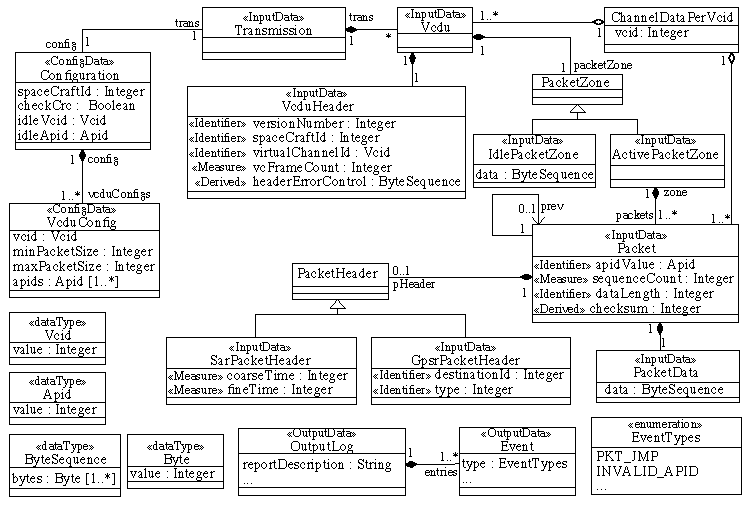
\includegraphics{images/classDiagramSmall}
%      \caption{Simplified input data model taken from~\cite{di2015evolutionary}.}
%      \label{fig:dataModel}
%\end{figure}
%
%\begin{figure}[h]
%  \centering
%    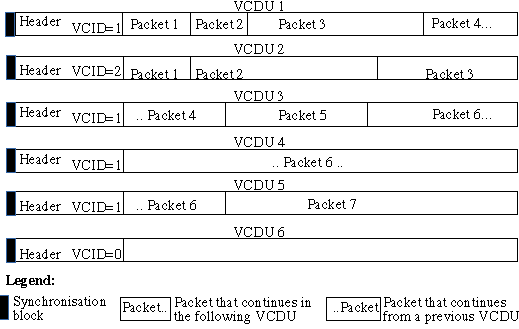
\includegraphics{images/transmissionData}
%      \caption{A simplified example of the transmission data modelled by the class diagram in Figure~\ref{fig:dataModel}.}
%      \label{fig:transmissionData}
%\end{figure}
%
%\begin{figure}[h]
%  \centering
%    \includegraphics{images/CADU}
%      \caption{Header of VCDU 3 followed by a portion of its packet zone.}
%      \label{fig:VCDU}
%\end{figure}
%
%\begin{figure}[h]
%  \centering
%    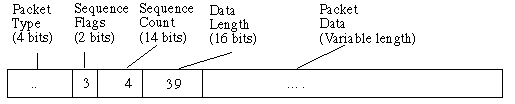
\includegraphics{images/packet}
%      \caption{Structure of a packet.}
%      \label{fig:packet}
%\end{figure}
%
%
%
%
%% An example fault model is described in Table~\ref{table:faultModel:SES}.
%%%and are used to identify the fields that can be mutated to generate new inputs.
%%For example, 
%%the two stereotypes \emph{Identifier} and \emph{Measure} are used to indicate that these attributes should be modified using mutation operators specified for identifiers and measurements.
%
%
%In the presence of UML models, constraints between inputs and outputs can be represented using OCL.
%These constraints are used as an oracle to validate the execution of automatically generated test cases: a violated constraint indicates that the system under test does not produce the expected output. 
%%The use of OCL constraints enable engineers to represent information that cannot be captured with grammars.
%%In the case of SES-DAQ, we use OCL constraints to model the error messages expected in the presence of specific faults in the input data.
%For example, Figure~\ref{fig:costraint:firstHeader} shows an OCL constraint that states that the frame count of a VCDU should be greater by one than the frame count of the previous VCDU on the same virtual channel. Otherwise, an error event \emph{COUNTER\_JUMP} should exist in the system output log file. 
%In the context of data-driven mutation testing they can be used to determine if a mutant had been killed by a test case (e.g., a constraint may capture the presence of a log entry indicting the triggering a redundancy mechanism).
%
%
%
%\begin{figure}[t!]
%\scriptsize
%\begin{tabular}{p{0.1cm}p{8cm}}
%1&\textbf{context} Vcdu \textbf{inv}:\\
%2&\textbf{let}\\
%3&\hspace{0.3cm}frameCount : Integer = self.header.vcFrameCount, \\
%4&\hspace{0.3cm}vdcuIndex : Integer = self.virtualChannel.vcdu$\rightarrow$indexOf( self ), \\
%5&\hspace{0.3cm}previous : Vcdu = self.virtualChannel.vcdu$\rightarrow$at( vcduIndex - 1 ),\\
%6&\hspace{0.3cm}previousFrameCount : Integer = previous.header.vcFrameCount\\
%7&\textbf{in} \\
%8&\hspace{0.3cm}\textbf{if} previousFrameCount $<$ 16777215 \\
%9&\hspace{0.6cm}\textbf{then} frameCount $<>$ previousFrameCount + 1 \\
%10&\hspace{0.3cm}\textbf{else} previousFrameCount $=$ 16777215 and frameCount $<>$ 0 \textbf{endif}\\
%11&\textbf{implies} \\
%12&\hspace{0.3cm}VcduEvents.allInstances()\\
%13&\hspace{1cm}$\rightarrow$exists(e $|$ e.eventType = $COUNTER\_JUMP$) \\
%\end{tabular}
%\caption{Input/output constraint for the \emph{COUNTER\_JUMP} error event.}
%\label{fig:costraint:firstHeader}
%\end{figure}
%
%
% 
%%The stereotype \emph{Derived} is used to tag class attributes that need to be derived from other attributes after every mutation, in order to prevent trivial inconsistencies (e.g. it is used to update the checksum field when other fields are mutated). 
%%The stereotypes \emph{StreamClass} and \emph{StreamAttributes} are used to automate the loading of data from bytestreams.
%% but are out of the scope of this paper (see~\cite{ICST15} for details).
%
%The main limitation of UML-based approaches is the lack of generalistic binary parsers capable of loading data as an instance of a UML class diagram. Existing approaches rely on custom parsers~\cite{di2015generating,di2015evolutionary}.
%
%\subsubsection{Data modeling with Block Models}
%
%Approaches relying on block models~\cite{PeachFuzzer,spike,pham2016model}, require that engineers specify input data according to a specific format that captures the size of specific portions of the input data. 
%For example, Spike~\cite{spike} and Peach~\cite{PeachFuzzer} require input models that specify the format of data chunks and integrity constraints.
%Figure~\ref{fig:pit} shows a portion of an example block model taken from related work~\cite{pham2016model}.
%While being effective in fuzzing programs that process weakly-structured inputs (e.g., images and protocols), these approaches become less effective for highly-structured inputs (e.g., JavaScript).
%Compared to UML-based modeling, block models provide more limited modeling capabilities, for instance, they are less effective for highly-structured inputs; however, they are often integrated into general-purpose tools that can be easily integrated in software projects~\cite{PeachFuzzer}.
%
%
%\begin{figure}[t!]
%  \centering
%    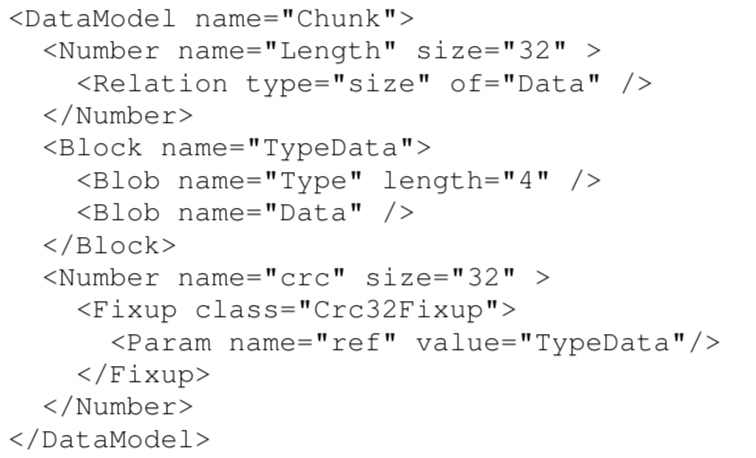
\includegraphics[width=7cm]{images/PeachPit}
%      \caption{Data model with a custom format.}
%      \label{fig:pit}
%\end{figure}
%
%
%%%%%%%%%%%%%%%%%%%%%%%%%%%%%%%%%%
%
%\subsection{Data-driven Mutation Operators}
%\label{sec:data_operators}
%
%%As mentioned in Section~\ref{sec:dataProcess}, the software engineering literature does not include any study on data-driven mutation testing but only testing approaches based on the injection of data faults.
%%For this reason, 
%In this section, we provide an overview of the fault injection techniques that have originally been developed to support software testing and can be used in the context of data-driven mutation testing. 
%More precisely, we focus on the techniques for the modification of data (hereafter, data mutation techniques) that are presented in software testing research papers.
%
%
%Table~\ref{table:dataOperators} provides an overview of groups of data mutation techniques that can be applied to space software and embedded systems. 
%We selected the set of data-driven mutation techniques in Table~\ref{table:dataOperators} based on the different types of faults commonly affecting space and embedded systems.
%Each technique aims to create data faults that might be observed in real systems either because of hardware errors or software errors.
%The data-driven mutation operators, i.e., the specific functions implemented by each technique to alter the type of data they target, are described in separate tables, in the following paragraphs. 
%%Since, for each family of technique, multiple implementations of data-driven mutation operators are available
%
%In Table~\ref{table:dataOperators}, column \emph{Name} provides the name of the specific technique described,  
% column \emph{Type of fault} indicates the type of faults each operator aims to simulate,
% column \emph{Data model} indicates if the technique requires a model of the structure of the data to be mutated,
% column \emph{Definition} provides a brief description of the technique, column \emph{Target} indicates the type of data targeted,
% column \emph{Reference} provides a reference to a research paper or tool describing the technique more in detail.
% 
%%Fabrizio: "First" and "Then" read like a story, which is not good in a Tech Report
%Concerning the type of faults considered, we focus both on hardware and software errors.
%Hardware errors are captured by the categories CPU Faults, Memory Faults, and Signal Faults. 
%Software errors are captured by the category Data Processing Faults.
%Category Communication Faults simulates problems that can be caused either by software or hardware errors.
%
%
%
%\newcommand{\FTAPE}{\cite{tsai1999stress}}
%\newcommand{\FIAT}{\cite{barton1990fault}}
%\newcommand{\GOOFI}{\cite{aidemark2001goofi}}
%\newcommand{\DOCTOR}{\cite{han1995doctor}}
%\newcommand{\ORCHESTRA}{\cite{dawson1996testing}}
%\newcommand{\Fuzz}{\cite{miller1995fuzz}}
%\newcommand{\Ballista}{\cite{koopman2000exception}}
%\newcommand{\RIDDLE}{\cite{ghosh1998testing}}
%\newcommand{\Superion}{\cite{Wang:GrammarAwareFuzzying:ICSE:2019}}
%\newcommand{\AFL}{\cite{gutmann2016fuzzing}}
%\newcommand{\SAGE}{\cite{godefroid2012sage}}
%\newcommand{\pFuzzer}{\cite{mathis2019parser}} 
%\newcommand{\MoWF}{\cite{pham2016model}}
%\newcommand{\DiNardoICST}{\cite{di2015generating}}
%\newcommand{\DiNardoASE}{\cite{di2015evolutionary}}
%\newcommand{\Matinnejad}{\cite{Matinnejad19}}
%\newcommand{\MongoDB}{\cite{Guo:MongoDBFuzzer:CACM:2017}}
%\newcommand{\SOLMI}{\cite{Jan:ISSTA:2016}}
%\newcommand{\MUSQL}{\cite{Appelt:SQLI:ISSTA:2014}}
%
%Table~\ref{table:dataMutation:references} provides the names of the tools and approaches referenced in Table~\ref{table:dataOperators}, along with a URL for the download of the tool, if available.
%
%% !TEX root =  ../MutationTestingSurvey.tex

\begin{table}[ht]
\tiny
\caption{Description of approaches and tools appearing in Table~\ref{table:dataOperators}.}
\begin{center}
\begin{tabular}{|p{1cm}|p{4cm}|p{8cm}|}
\hline
\textbf{Reference} & \textbf{Approach and Tool name} & \textbf{Available} \\
\hline

\cite{di2015evolutionary}	& Di Nardo et al. Search-based Mutation & No \\
\cite{di2015generating} & Di Nardo et al. Model-based Mutation & No \\
\cite{Matinnejad19} & Matinnejad et al. Signal Mutation & No \\

\cite{tsai1999stress} & FTAPE & No\\
\cite{barton1990fault} & FIAT & No \\
\cite{han1995doctor} & DOCTOR & No \\
\cite{dawson1996testing} & ORCHESTRA & No \\

\cite{miller1995fuzz} & Fuzz & Yes, \url{http://pages.cs.wisc.edu/~bart/fuzz/fuzz.html} \\


\cite{koopman2000exception}	&  Ballista & Yes, \url{http://users.ece.cmu.edu/~koopman/ballista/} \\

%\cite{ghosh1998testing}	& RIDDLE & No \\
\cite{Wang:GrammarAwareFuzzying:ICSE:2019} & Superion & \url{https://github.com/zhunki/Superion} \\
\MongoDB	& MongoDB Fuzzer & No \\
\SOLMI	& SOLMI &No \\
\MUSQL	& \emph{$\mu$4SQLi} &No\\
\cite{gutmann2016fuzzing} & American Fuzzy Lop & Yes, \url{https://github.com/google/AFL}\\
\cite{godefroid2012sage} & SAGE & \begin{tabular}[c]{@{}l@{}}Yes, now under Microsoft Security Risk Detection service\\\url{https://www.microsoft.com/en-us/security-risk-detection/}\end{tabular} \\
%\cite{mathis2019parser}	& pFuzzer & Yes, \url{https://github.com/uds-se/pFuzzer}\\
\cite{pham2016model} &	MoWF & No \\
\cite{spike}&SPIKE&\url{https://github.com/guilhermeferreira/spikepp}\\
\cite{PeachFuzzer}&PEACH&\url{https://www.peach.tech}\\
\cite{BooFuzz}&BooFuzz&\url{https://github.com/jtpereyda/boofuzz}\\
\hline
\end{tabular}
\end{center}
\label{table:dataMutation:references}
\end{table}%


%
%% !TEX root =  ../MutationTestingSurvey.tex

\newcommand{\FTAPE}{\cite{tsai1999stress}}
\newcommand{\FIAT}{\cite{barton1990fault}}
\newcommand{\GOOFI}{\cite{aidemark2001goofi}}
\newcommand{\DOCTOR}{\cite{han1995doctor}}
\newcommand{\ORCHESTRA}{\cite{dawson1996testing}}
\newcommand{\Fuzz}{\cite{miller1995fuzz}}
\newcommand{\Ballista}{\cite{koopman2000exception}}
\newcommand{\RIDDLE}{\cite{ghosh1998testing}}
\newcommand{\AFL}{\cite{gutmann2016fuzzing}}
\newcommand{\SAGE}{\cite{godefroid2012sage}}
\newcommand{\pFuzzer}{\cite{mathis2019parser}} 
\newcommand{\MoWF}{\cite{pham2016model}}
\newcommand{\DiNardoICST}{\cite{di2015generating}}
\newcommand{\DiNardoASE}{\cite{di2015evolutionary}}
\newcommand{\Matinnejad}{\cite{Matinnejad19}}

\begin{itemize}
	\item FTAPE tool: \cite{tsai1999stress}
	\item FIAT tool: \cite{barton1990fault}
	\item GOOFI tool: \cite{aidemark2001goofi}
	\item DOCTOR tool: \cite{han1995doctor}
	\item ORCHESTRA tool: \cite{dawson1996testing}
	\item Fuzz tool:\cite{miller1995fuzz}
	\item Ballista tool: \cite{koopman2000exception}
	\item RIDDLE tool: \cite{ghosh1998testing}
	\item American Fuzzy Lop tool: \cite{gutmann2016fuzzing}
	\item SAGE tool: \cite{godefroid2012sage}
	\item pFuzzer tool: \cite{mathis2019parser}
	\item MoWF tool: \cite{pham2016model}
	\item Di Nardo et al. Model-based Mutation tool: \cite{di2015generating}
	\item Di Nardo et al. Search-based Mutation tool: \cite{di2015evolutionary}
	\item Matinnejad et al. Signal Mutation tool: \cite{Matinnejad19}
\end{itemize}

\tiny
\setlength\LTleft{0pt}
\setlength\LTright{0pt}
\begin{longtable}{@{\extracolsep{\fill}}|p{1.5cm}|p{2cm}|p{5cm}|p{3cm}|p{1cm}|@{}}
\toprule
	\textbf{Name}	&	\textbf{Type of Fault}	&	\textbf{Definition}	&	\textbf{Target}	&	\textbf{Reference} \\
	\midrule
stuck-at-0 & CPU Faults; Memory Faults & This operator corrupts data by replacing a bit/byte/word with zero. & CPU registers; Memory registers & \FTAPE, \FIAT, \GOOFI \\
stuck-at-1 & CPU Faults; Memory Faults & This operator corrupts data by replacing a bit/byte/word with one. & CPU registers; Memory registers & \FTAPE, \FIAT, \GOOFI \\
bit flips & CPU Faults; Memory Faults; Data Processing Faults & This operator mutates data by inverting the value of each bit (i.e., replacing 0 with 1 and 1 with 0). & CPU registers: saved registers, floating point registers, the program counter, global pointer, stack pointer; Local memory; Input or output parameters of a software interface. & \FTAPE, \FIAT, \GOOFI \\
disk driver codes & Communication Faults & This operator performs data mutation by modifying the error flags of a disk driver. & I/O disk driver codes. & \FTAPE \\
set & CPU Faults; Communication Faults; Memory Faults & This operator sets the value of a bit/byte by replacing the current value with one or a user-defined bitmap. & Memory: stack, heap, global data, user code, user-defined memory location; Registers: data, stack, address, program counter, status register & \FTAPE, \FIAT, \GOOFI \\
clear & CPU Faults; Communication Faults; Memory Faults & This operator clears the value of a bit/byte by replacing the current value "v" with zero. & Memory: stack, heap, global data, user code, kernel code, user-defined memory location; Registers: data, stack, address, program counter, status register & \FTAPE, \FIAT, \GOOFI \\
toggle & CPU Faults; Communication Faults; Memory Faults & This operator toggles (i.e., sets a bit to its complement state) a bit/byte. & Memory: stack, heap, global data, user code, kernel code, user-defined memory location; Registers: data, stack, address, program counter, status register & \FTAPE, \FIAT, \GOOFI \\
lose message & Communication Faults & This operator causes a message to be lost in between two communicating components. Messages can be lost intermittently, with a probability distribution specified by the users, or alternatively, every message can be lost during a certain period. & Faulty link, Faulty direction, Single message & \DOCTOR, \ORCHESTRA \\
duplicate message & Communication Faults & This operator causes a message to be duplicated in between two communicating components. & Faulty link, Faulty direction, Single message & \DOCTOR, \ORCHESTRA \\
alter message header & Communication Faults & This operator alters a message. The change is performed in a similar manner as for memory faults, i.e., by performing bit flips. The mutation is performed in the message header. & Faulty link, Faulty direction, Single message & \DOCTOR, \ORCHESTRA \\
alter message body & Communication Faults & This operator alters a message. The change is performed in a similar manner as for memory faults, i.e., by performing bit flips. The mutation is performed in the message body. & Faulty link, Faulty direction, Single message & \DOCTOR, \ORCHESTRA \\
delay message & Communication Faults & This operator causes a message to be delayed in between two communicating components. The delay time can either be constant or follow a probability distribution. & Faulty link, Faulty direction, Single message & \DOCTOR, \ORCHESTRA \\
fuzzing & Data Processing Faults & Fuzzing techniques replace values with values (i.e., fuzz values) that are different and, usually, randomly generated. & Structured input data (e.g., files, streams) & \Fuzz, \Ballista \\
grammar-based fuzzing & Data Processing Faults & This fuzzing approach relies on a grammar that describes the format of the data to be altered; new values are generated according to the grammar. The use of the grammar decreases the chances of generating invalid inputs. & Structured input data (e.g., files, streams) & \RIDDLE \\
evolutionary fuzzing & Data Processing Faults & This fuzzing approach relies on evolutionary algorithms (e.g., genetic algorithms) to generate fuzz values. It relies on a fitness function to maximize structural coverage (e.g., branches executed during testing). The fitness is implemented by instrumenting the code of the application to collect code coverage. & Structured input data (e.g., files, streams) & \AFL \\
whitebox fuzzing & Data Processing Faults & This fuzzing approach relies on symbolic execution techniques to cover corners cases on the different execution paths. & Structured input data (e.g., files, streams) & \SAGE \\
parser-directed fuzzing & Data Processing Faults & Fuzzing techniques replace a correct value with a randomly generated one. This fuzzing operator is applied to programs that integrate a parser component to extract information from the provided inputs. It is implemented through a test generator technique that aims to produce valid inputs for the parser, the inputs are produced randomly and then checked using constraint solving techniques. & Structured input data (e.g., files, streams) & \pFuzzer \\
model-based whitebox fuzzing & Data Processing Faults & Fuzzing techniques replace a correct value with a randomly generated one, in this case, the replacement is done using a model-based whitebox fuzzing technique, the technique prunes from the search space those paths that are exercised by invalid, malformed inputs. The model should specify the format of the data chunks and integrity constraints. & Structured input data (e.g., files, streams) & \MoWF \\
data-type based injection & Data Processing Faults & This operator replaces a value with an invalid one, selected on the basis of the type of the parameter being corrupted. & Structured input data (e.g., files, streams) & \Fuzz, \Ballista, \RIDDLE \\
model-based mutation & Data Processing Faults & This approach alters existing inputs by relying on a data model that capture the structure of the data and the constraints among data fields. A predefined set of operators indicating how to alter data based on its structure are provided. & Structured input data (e.g., files, streams) & \DiNardoICST \\
search-based data mutation & Data Processing Faults & This approach alters existing inputs by relying on a data model that captures the structure of the data and the constraints between data fields. A search-based, evolutionary algorithm is used to maximize a number of mutation objectives including the number of constraints being violated and code coverage. & Structured input data (e.g., files, streams) & \DiNardoASE \\
signal mutation & Signal faults & This approach alters signal by either shifting the signal based on a randomly selected value or shifting the signal and increasing the number of signal pieces (i.e., segments).  & Input signals & \Matinnejad \\

	\bottomrule                                                             
\caption{Data-driven Mutation Operators.}
\label{table:dataOperators}
\end{longtable}
\normalsize
%
%To summarize the data in Table~\ref{table:dataOperators}, we observe that:
%\begin{itemize}
%  %Note: always put a comma at the end of a list before "or" "and"
%  \item Category CPU Faults includes techniques that perform mutations in the contents of an individual bit, byte, or word in a CPU register. The mutations in this category can target saved, floating-point, program-counter, global and stack-pointer register locations. 
%  \item Category Memory Faults includes techniques that perform mutations in the contents of an individual bit, byte, or word in a memory register. The mutations in this category can target stack, heap, global-data and user-defined memory locations.
%  \item Category Communication Faults includes techniques that simulate packet corruption faults. The mutations in this category can target channels between components, single messages, and the addresses of the messages to be exchanged.
%  \item Category Data Processing Faults includes techniques that mutate the data being processed by the system. Some of these techniques are white-box, they process the source code of the application to generate inputs more efficiently. Other techniques require a model of the data to be mutated. The mutations in this category can target both the input and the output parameters of the interface of a software component.
%  \item Category Signal Faults includes techniques that alter the shape of the signals received by the software under test.
%\end{itemize}
%
%In the following, we provide an overview of the mutation operators implemented by the most representative techniques.
%We do not present simple fuzzing approaches because they simply perform random mutations and they include a subset of the operators implemented in the more advanced evolutionary fuzzing approaches.
%
%\subsubsection{Blind memory corruption and blind transmission corruption}
%
%The mutation operators implemented by techniques performing blind memory corruption and blind transmission corruption are presented in Tables~\ref{table:operators:blindTransmissions} and ~\ref{table:operators:blindTransmissions}, respectively. These techniques do not require a data model. Unfortunately, they are of little usefulness to simulate subtle errors that affect relations among data (e.g., replacing an identifier with another legal one).
%
%%Among all the data mutation operators reported in Table~\ref{table:dataOperators}, the ones targeting \emph{Data Processing Faults} are more powerful since they concern the modification of complex data structures. %Oscar: not sure that "overviewed" is spelled right %They are briefly overviewed in the following.
%%We provide an overview in the following.
%
%
%\subsubsection{Evolutionary Fuzzing}
%
%
%%\subsubsection{Approaches generating data from scratch}
%AFL is an instrumentation-guided fuzzer~\cite{gutmann2016fuzzing}. It integrates genetic algorithms with a form of branch coverage called state transition coverage,
%which captures the number of times each branch is taken in an execution. 
%AFL aims to generate inputs that exercise all the different code paths.
%%It is implemented by executing for every instruction of the program under test the following lines
%%cur_location = <COMPILE_TIME_RANDOM>;
%%coverage[cur_location ^ prev_location]++; 
%%prev_location = cur_location >> 1;
%It requires one or more starting files that contain input data normally processed by the targeted application. 
%Each provided input is processed in a queue. For each input in the queue, AFL trims the test case to the smallest size that doesn't alter the coverage of the program. Then it repeatedly mutates the file using a set of fuzzing strategies, which are presented in Table~\ref{table:AFL:operators}.
%If any of the generated mutations result in a change of the coverage for the software under test, the mutated input is added to the input queue.
%
%% !TEX root =  ../MutationTestingSurvey.tex

%
%\setlength\LTleft{0pt}
%\setlength\LTright{0pt}
%\begin{longtable}{@{\extracolsep{\fill}}|p{2.5cm}|p{5cm}|p{5cm}|@{}}
%\toprule


\begin{table}[h]
\caption{Mutation Operations performed by AFL~\cite{gutmann2016fuzzing}}
\label{table:AFL:operators}


\tiny
\begin{tabular}{|p{2.5cm}|p{10cm}|}

\hline

\textbf{Walking bit flips}& Sequential, ordered bit flips. The number of bits flipped in a row varies from one to four in steps of two. This strategy is applied till the coverage of the program under test does not change.\\

\hline
\textbf{Walking byte flips}& This method relies on 8-, 16-, or 32-bit wide bitflips with a constant stepover of one byte. \\

\hline
\textbf{Simple arithmetics}& Increment and decrement existing integer values in the input file; this is done considering every byte of the file. The chosen range for the operation is -35 to +35. It is performed in three steps. First, the fuzzer attempts to perform subtraction and addition on individual bytes. The second steps involves looking at 16-bit values, using both endians - but incrementing or decrementing them only if the operation has affected the most significant byte. The final stage follows the same logic, but for 32-bit integers.\\

\hline
\textbf{Known integers}& 
AFL overwrites every byte in the input file with a set of interesting values (e.g., -1, 256, 1024, MAX\_INT-1, MAX\_INT), using both endians (the writes are 8-, 16-, and 32-bit wide).\\

\hline
\textbf{Stacked tweaks}& Sequence of randomly selected mutations among the following: Single-bit flips, Attempts to set "interesting" bytes, words, or dwords (both endians), Addition or subtraction of small integers considering bytes, words, or double words (both endians), Random single-byte sets, Block deletion, Block duplication via overwrite or insertion, Block memset. \\

\hline
\textbf{Test case splicing}& Consists of taking two distinct input files that differ in at least two locations, splicing them at a random location in the middle, and then applying stacked tweaks.\\

\hline
%\bottomrule                                                             

\end{tabular}
\end{table}
%\normalsize



%
%\subsubsection{Grammar-based fuzzing}
%
%Superion~\Superion~ extends \emph{AFL} to drive mutations based on grammars. It takes as input an ANTLR~\cite{ANTLR} grammar. 
%It performs mutations that consist of grammar-aware trimming, dictionary-based mutations, and tree-based mutation.
%Grammar-aware trimming is performed by generating an AST tree from the input and by deleting a randomly-selected subtree. 
%It aims to generate trimmed inputs that do not alter code coverage in the SUT.
%Dictionary-based mutations are performed by building a dictionary using every token in the input file and by inserting the elements of the dictionary in the boundaries of every token in the input file.
%Tree-based mutation is performed by processing two input files and replacing the subtrees of one file with the ones of another.
%Listing~\ref{mutatedJSONfile} shows a JSON file generated by deleting a randomly-selected subtree from Listing~\ref{JSONfile}.
%
%
\begin{minipage}{14cm}
\footnotesize
\begin{lstlisting}[caption=JSON file generated by deleting a subtree from Listing~\ref{JSONfile}., label=mutatedJSONfile]
{
 [
 {
  "firstName": "Fabrizio",
  "lastName": "Pastore",
  "isAlive": true,
  },
  {
  "firstName": "Oscar",
  "lastName": "Cornejo",
  "isAlive": true,
  "address": {
    "streetAddress": "29, Avenue J.F Kennedy",
    "city": "Luxembourg",
    "state": "Luxembourg",
    "postalCode": "L-1855"
  },
  }
  ]
}
\end{lstlisting}
\end{minipage}
%
%%Fabrizio: you had this definition of equivalent: "(i.e., correct fuzzed data, but semantically meaningless)." it is difficult to understand
%
%
%%Fabrizio: I cannot understand the following sentences
%%Although it tackles the problem of redundant mutants by well covering the space of possible inputs, it does not tackle the redundant mutant problem.
%%Cannot handle semantic restrictions imposed by certain nontrivial input languages. The approach has difficulties to handle complex sequences recursion.
%
%%\subsubsection{Approaches altering existing data}
%
%
%\emph{$\mu$4SQLi}~\cite{Appelt:SQLI:ISSTA:2014} relies on a SQL grammar to generate SQL injections. 
%SQL injections are generated by means of a set of mutation operators, shown in Table~\ref{table:Mu4SQLI}, that alter the values of an input according to predefined patterns.
%Similarly, SOLMI~\cite{Jan:ISSTA:2016} relies on the XML grammar to alter XML messages based on a predefined set of mutation operators and introduce potential XML injections. 
%SOLMI implements four operators that (1) introduce XML meta-characters, (2) introduce closing tags, (3) replicate XML elements, (4) replace XML content.
%
%
%\begin{table}[h]
%\caption{Mutation operators implemented by $\mu$4SQLi}
%\label{table:Mu4SQLI}
%\begin{tabular}{|p{2cm}|p{11.5cm}|}
%\hline
%\multicolumn{2}{|c|}{Behaviour-Changing Operators}\\
%\hline
%MO\_or&Adds an OR-clause to the input\\
%MO\_and&Adds an AND-clause to the input\\
%MO\_semi&Adds a semicolon followed by an additional SQL statement\\
%\hline
%\multicolumn{2}{|c|}{Syntax-Repairing Operators}\\
%\hline
%MO\_par&Appends a parenthesis to a valid input\\
%MO\_cmt&Adds a comment command (- - or \#) to an input\\
%MO\_qot&Adds a single or double quote to an input\\
%\hline
%\multicolumn{2}{|c|}{Obfuscation Operators}\\
%\hline
%MO\_wsp&Changes the encoding of whitespaces \\
%MO\_chr&Changes the encoding of a character literal enclosed in quotes\\
%MO\_html&Changes the encoding of an input to HTML entity encoding\\
%MO\_per&Changes the encoding of an input to percentage encoding\\
%MO\_bool&Rewrites a boolean expression while preserving its truth value\\
%MO\_keyw&Obfuscates SQL keywords by randomising the capitalisation and inserting comments\\
%\hline
%\end{tabular}
%\end{table}
%
%
%Tal et al.~\cite{Tal2004} presented a syntax-based vulnerability testing technique based on mutations of ASN.1 grammars. The objective is to detect software vulnerabilities detecting anomalous behavior or crashes in the SUT (e.g., segmentation faults, buffer, heap or stack overflows, etc.) when parsing mutated PDUs. The PDUs are specified by frames (data structures), which explicitly defines the order of data fields in the PDU, as well as the exact length of each field. 
%The proposed approach intercepts OSPF packets and translates it to a TXL readable file, then the mutations are applied to ASN.1 syntax contained in the TXL file. The mutation strategies applied are the following: \textbf{replacement} (replacing one field at a time with boundary and mid-way values), \textbf{removal} (removing one field at a time, and then removing pairs of fields, one pair at a time), and \textbf{permutation} (permutating pairs of fields within each SEQUENCE and SET).
%
%% \textbf{Syntax-based Vulnerability Testing of Frame-based Network Protocols}
%% \cite{Tal2004} The paper presents a syntax-based vulnerability testing technique based on mutations of Protocol Data Units (PDU) performed on the ASN.1 syntax. The objective is to detect software vulnerabilities detecting anomalous behavior or crashes in the SUT (e.g., segmentation faults, buffer, heap or stack overflows, etc.) when parsing mutated PDUs. The PDUs are specified by frames (data structures), which explicitly defines the order of data fields in the PDU, as well as the exact length of each field.
%% Syntax is specified in BNF notation, mutations are then made to the syntactic elements and the grammar is used to produce mutated vectors (PDUs). In the paper, the transferred packets are based on the OSPF protocol. Previously, it has been applied to WAP, HTTP, LDAP and SNMP protocols.
%% The proposed approach intercepts a packet and translates it to a TXL readable file, then the mutations are applied to ASN.1 syntax contained in the TXL file. The mutation strategies applied are the following: replacement (replacing one field at a time with boundary and mid-way values), removal (removing one field at a time, and then removing pairs of fields, one pair at a time), and permutation (permutating pairs of fields within each SEQUENCE and SET).
%
%
%% \textbf{CMM: A combination-based mutation method for SQL injection}
%
%Instead, Zhao et al.~\cite{Zhao2020} presented a mutation-based fuzzing technique for eliminating SQLi vulnerabilities. The technique is called Combinatorial Mutation Method (CMM), which mixes combinatorial testing with fuzzing techniques to generate test sets for SQLi. 
%
%The mutations are based on the mutation methods from sqlmap (open source penetration testing tool that automates the process of detecting and exploiting SQLi flaws). The authors classifies the mutation methods provided by sqlmap in five groups:
%
%
%\begin{table}[h!]
%\begin{center}
%\begin{tabular}{|p{2cm}|p{10cm}|}
%\hline
%\textbf{Fault}&\textbf{Description}\\
%\hline
%comment & attach a sql comment command at the back of an input test case.\\
%stringtamper & changes the appearance of an input, making it look valid but still malicious. \\
%space2 & changes the space character in the input.\\
%apostle& changes the apostle in the input.\\
%encoding& this kind of mutation method changes the encoding of the original statement.\\
%\hline
%\end{tabular}
%\end{center}
%\caption{Fault Model from \cite{Zhao2020}}
%\label{table:faultModel:Zhao2020}
%\end{table}%
%
%The test set is created by using combinatorial testing on the different inputs created by the mutation tool.
%
%
%
%%\textbf{Testing for software vulnerability using environment perturbation}
%
%Du et al.~\cite{Du2002} introduced a fault injection technique to perform environment perturbations for testing a software system for possible security flaws. The paper introduces a fault model called Environment-Application Interaction (EAI).
%
%Given the assumption that a system is composed of an application plus its environment, in the paper faults are injected into the environment thereby perturbing it, the idea is to verify if the program responds and whether there will be a security violation under this perturbation, otherwise the system is considered secure.
%
%The faults are injected at the points where the environment and the application interact. The environment faults becomes faults in the input, which is then inherited by an internal entity of the application. From this point onwards the environment faults propagate through the application via the internal entities. If the application does not handle the faults correctly, a security violation might occur. The direct reason for this violation appears to be faults in the internal entity. 
%Authors classify environment faults in two categories: (1) indirect: affect programs via internal entities (primary sources of program inputs). (2) direct: affect programs via environment faults.
%
%
%\begin{figure}[h]
%  \centering
%    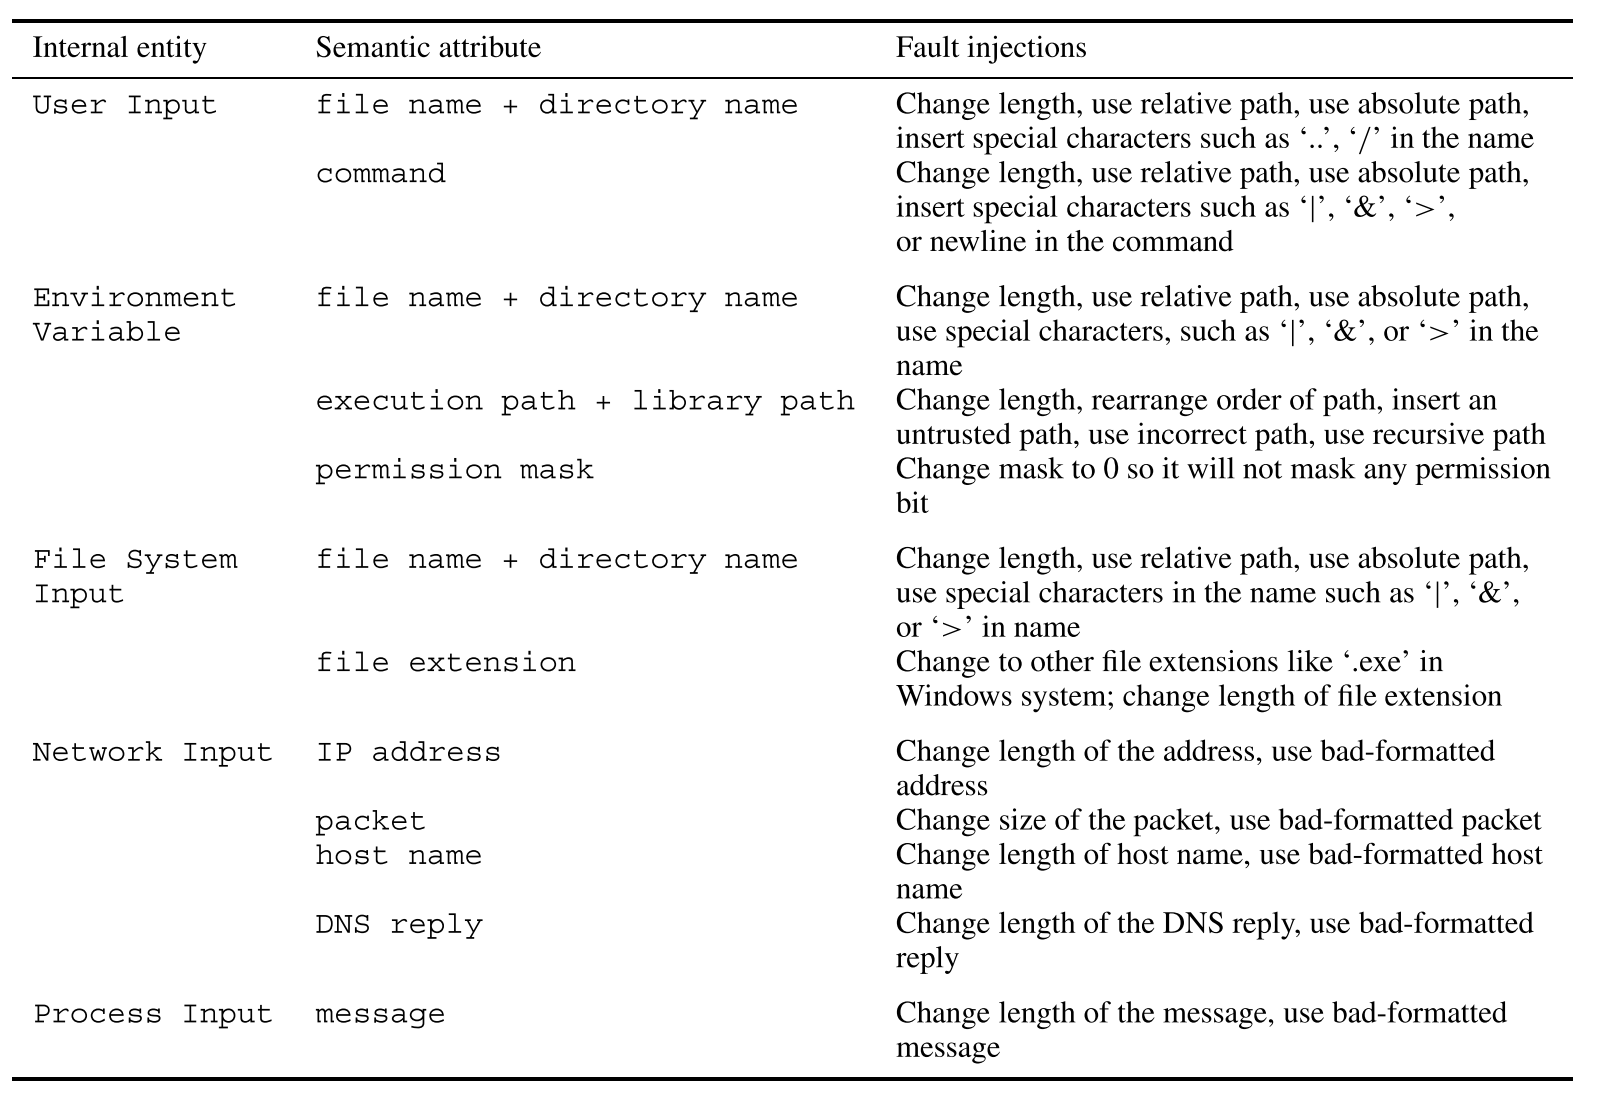
\includegraphics[width=0.8\textwidth]{images/du2002a}
%      \caption{Indirect environment faults and environment perturbations operators.}
%\end{figure}
%
%
%\begin{figure}[h]
%  \centering
%    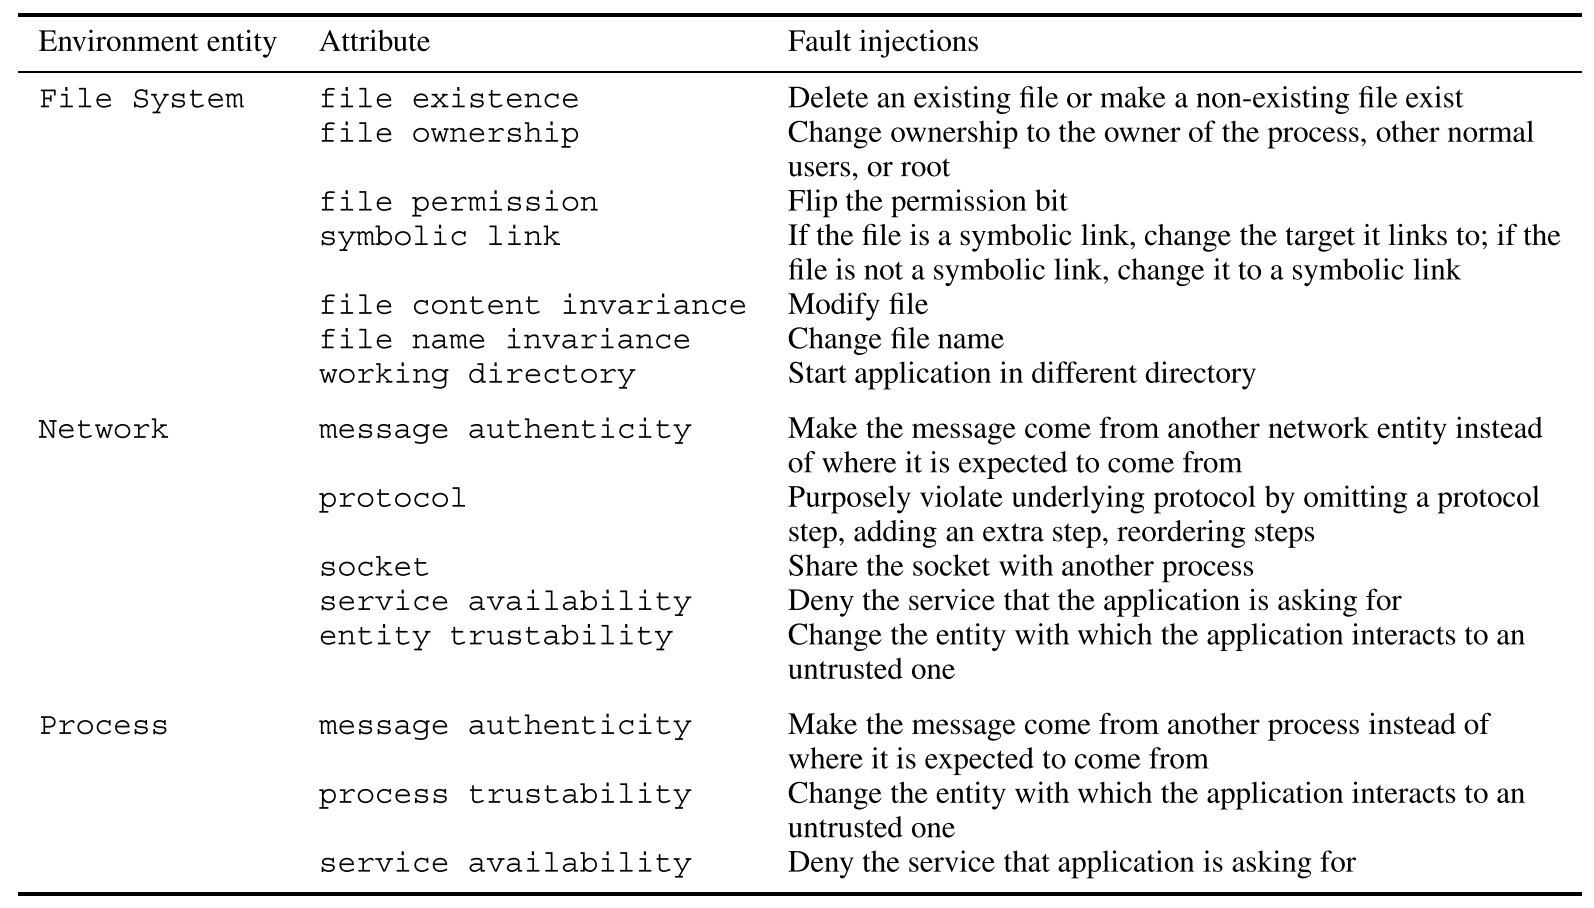
\includegraphics[width=0.8\textwidth]{images/du2002b}
%      \caption{direct environment and environment perturbations operators.}
%\end{figure}
%
%They use fault coverage (percentage of the number of faults tolerated to the faults injected) and interaction coverage (percentage of the number of interaction points where faults are injected w.r.t to total of interaction points) to measure the test adequacy.
%
%
%
%One of the major limitations of grammar-based approaches is the cost of defining an input grammar. MongoDB's javascript fuzzer addresses the problem of grammar-based mutation when a grammar is not available. Instead of mutating input files for the SUT based on the input grammar of  the SUT, it mutates test cases for the SUT (in this case the Javascript test cases)~\MongoDB. It replaces subtrees in the AST tree generated from the test cases either other subtrees belonging to the same input file or with subtrees generated following encoded production rules.
%
%
%
%
%
%\subsubsection{Whitebox fuzzing}
%
%%, also, it requires more knowledge about the target than purely random ones.
%
%SAGE adopts symbolic execution to systematically generate malformed inputs~\cite{godefroid2012sage}. SAGE performs fuzzing on file- and packet-parsing applications. 
%The program is first executed with concrete inputs; in order to identify a set of constraints on inputs, then, one of the constraints in the set is negated, and new malformed inputs are generated to satisfy the new set of constraints. 
%The main benefit of SAGE is that it forces the program to execute corner cases not covered by the initial inputs; for example, 
%%Fabrizio: you wrote the following, which I could not understand please check if my sentence is correct
%%(e.g., reached one-third of all bugs found by fuzz testing in Microsoft projects \cite{bounimova2013billions}).
%%Oscar: yes, what you wrote is correct 
%one-third of all the bugs found by means of fuzz testing are detected thanks to SAGE \cite{bounimova2013billions}.
%Unfortunately, the main limitation of SAGE and symbolic execution-based fuzzers is its limited scalability, due to the high execution time required by symbolic execution.
%
%%Fabrizio: not sure what the following is about, ignoring
%%\emph{Testing of Fault-Tolerant and Real-Time Distributed Systems via Protocol Fault Injection \cite{dawson1996testing}}: The paper introduces a portable fault injection environment for testing implementations of distributed protocols.
%
%\subsubsection{Model-based fuzzing}
%
%%Fabrizio: we miss the pro/cons from the following
%Model-based fuzzing targets program binaries that process structured inputs.
%Model-Based Blackbox Fuzzing (MoBF) is performed using block models that capture the structure of the input data for the SUT. A solution to perform MoBF is Peach~\cite{PeachFuzzer,PeachMozilla}, which alters data of an input files according to a large, predefined set of rules. We provide an overview of the mutation operators implemented by Peach in Table~\ref{table:PeachOperators}.
%Model-Based Whitebox Fuzzing, instead, relies on additional information about code coverage to generates valid inputs that exercise critical target locations~\cite{pham2016model}. This is done through a directed path exploration technique that prunes from the search space those paths that are exercised by invalid, malformed inputs.
%Compared with a Model-Based Blackbox Fuzzer (MoBF) approach, the \emph{MoWF} prototype was able to expose all of 13 vulnerabilities on an empirical evaluation carried on nine subject programs, while the MoBF approach only detected 6 out of 13 vulnerabilities. 
%
%% !TEX root = ../MutationTestingSurvey.tex

\begin{table}[h]
\begin{center}
\footnotesize
\CHANGEDTWO{
\begin{tabular}{|p{5cm}|p{9cm}|}
\hline
\textbf{Operator Name}&\textbf{Description}\\
\hline
ArrayVarianceMutator&Change the length of arrays. Given L the original length of the array, the length is changed in range L-N to L+N.\\
ArrayReverseOrderMutator&Reverse the order of an array.\\
ArrayRandomizeOrderMutator&Put array elements in random order.\\
DWORDSliderMutator&Slides a DWORD through the blob.\\
BitFlipperMutator&Flips a given \% of bits in blob. Default is 20\%.\\
BlobMutator&Randomly grows a Blob block or shrinks it.\\
DataTreeRemoveMutator&Remove nodes from data tree.\\
DataTreeDuplicateMutator&Duplicate a node's value starting at 2x through 50x.\\
DataTreeSwapNearNodesMutator&Swap the data of two nodes that are near each other in the data model.\\
NumericalVarianceMutator&Produce numbers that are defaultValue - N to defaultValue + N.\\
NumericalEdgeCaseMutator&Replace with random numbers of appropriate correct size.\\
FiniteRandomNumbersMutator&Produce a finite number of random numbers for each \emph{Number} element.\\
NumericalEvenDistributionMutator&Generate numbers evenly distributed through the total numerical space of the number range.\\
NullMutator&Does nothing, just test the data produced by the fuzzer.\\
PathValidationMutator&Does not mutate. Used to trace path of each test for path validation.\\
SizedVarianceMutator&Change the length of sizes to count - N to count + N.\\
SizedNumericalEdgeCasesMutator&Change the length of sizes to numerical edge cases.\\
SizedDataVarianceMutator& Change the length of sized data to count - N to count + N. Size indicator will stay the same.\\
SizedDataNumericalEdgeCasesMutator&Change the length of sizes to numerical edge cases.\\
StringCaseMutator&Change the case of a string.\\
UnicodeStringsMutator&Generate unicode strings.\\
ValidValuesMutator&Replace with random values other than the legal ones.\\
UnicodeBomMutator&Injects BOM markers into default value and longer strings.\\
UnicodeBadUtf8Mutator&Generate bad UTF-8 strings.\\
UnicodeUtf8ThreeCharMutator&Generate long UTF-8 three byte strings.\\
StringMutator&Generate a random unicode string, for each string node, one Node at a time.\\
XmlW3CMutator&Replace XML trees with invalid, non-well former, and valid (but random) XML trees.\\
PathMutator&Replace a path with an erroneous path generated according to 20 different rules.\\
HostnameMutator&Replace a hostname with an erroneous hostname generated according to 20 different rules.\\
IpAddressMutator&Replace an IP address with an erroneous IP address generated according to 20 different rules.\\
TimeMutator&Replace a time value with an erroneous value generated according to 3 different rules.\\
DateMutator&Replace a date with 60 predefined erroneous dates.\\ 
FilenameMutator&Replace a file name with an file name generated according to 10 different rules.\\
ArrayNumericalEdgeCasesMutator&This operator is not well documented in the source code of Peach.\\
BlobSpread&This operator is not well documented in the source code of Peach.\\
\hline
\end{tabular}
}
\end{center}
\caption{Mutation Operators for the opensource version of Peach~\cite{PeachMozilla}}
\label{table:PeachOperators}
\end{table}%
%
%\subsubsection{Model-based data mutation}
%
%%\emph{Generating complex and faulty test data through model-based mutation analysis (Research paper) \cite{di2015generating}}: 
%Model-based data mutation testing concerns the automated generation of invalid input data through the mutation of existing data based on a predefined set of mutation operators~\cite{di2015generating}.
%The technique receives two inputs: field data and a data model, i.e., a UML class diagram annotated with stereotypes and OCL constraints. 
%An example data model has been shown in Figure~\ref{fig:dataModel} while an example OCL constraint appears in Figure~\ref{fig:costraint:firstHeader}. 
%The technique relies upon six generic mutation operators to automatically generate faulty data. 
%Table~\ref{table:dataModelMutationOperators} provides an overview of the mutation operators proposed in ~\cite{di2015generating}.
%In model-based data mutation~\cite{di2015generating} stereotypes are used to tailor the behaviour of the generic mutation operators to the fault model for the system under test and the environment in which it is deployed. 
%Table~\ref{table:faultModel:SES} shows a fault model for a satellite system that processes the data presented in Figure~\ref{fig:dataModel}.
%Mutation operators are applied to the data according to the stereotypes used in the data model.
%Table~\ref{table:mapping} shows the mutation operators and the corresponding stereotypes. In~\cite{di2015generating}, the mutation operator \emph{Attribute Bit Flipping} is applied on all the attributes not tagged with other stereotypes. 
%
%\begin{table}[h]
\begin{center}
\begin{tabular}{|p{5cm}|p{5cm}|p{2.5cm}|}
\hline
\textbf{Fault}&\textbf{Mutation Operator}&\textbf{Stereotype}\\
\hline
Duplicate VCDU/Packet& Class Instance Duplication.&InputData\\
Missing VCDU/Packet& Class Instance Removal.&InputData\\
Wrong Sequence& Class Instances Swapping.&InputData\\
Incorrect Identifier& Attribute Replacement with Random.&Identifier\\
Incorrect Checksum& Attribute Replacement with Random.&Identifier\\
Incorrect Counter& Attribute Replacement using Boundary Condition.&Measure\\
Flipped Data Bits& Attribute Bit Flipping.&\\
\hline
\end{tabular}
\end{center}
\caption{Mapping between Fault Data and Mutation Operators in \cite{di2015generating}.}
\label{table:mapping}
\end{table}%
%
%% !TEX root =  ../MutationTestingSurvey.tex

%
%\setlength\LTleft{0pt}
%\setlength\LTright{0pt}
%\begin{longtable}{@{\extracolsep{\fill}}|p{2.5cm}|p{5cm}|p{5cm}|@{}}
%\toprule


\begin{table}[h]
\caption{Mutation Operators for Model-based Data-driven Mutation Testing. Based on~\cite{di2015generating}}
\label{table:dataModelMutationOperators}


\tiny
\begin{tabular}{|p{2.5cm}|p{5cm}|p{7cm}|}

\hline
\textbf{Operator}&\textbf{Description}&\textbf{Example}\\
\hline
\textbf{Class Instance Duplication (CID)}&
The operator \emph{Class Instance Duplication} duplicates an instance of a class belonging to a collection of elements. This operator copies a randomly chosen instance of a class in a collection and then inserts it at a random position in the collection. This operator simulates unexpected data in a collection.
&In Figure~\ref{fig:dataModel}, this operator can be applied to the associations between the classes \emph{Transmission} and \emph{Vcdu}, and between the classes \emph{VirtualChannel} and \emph{Packet}. In both cases the duplicated data generated by this operator simulates a transmission error.\\
\hline
\textbf{Class Instance Removal (CIR)}
&This mutation operator deletes a randomly selected instance of a class from a collection of elements. 
&In Figure~\ref{fig:dataModel}, this operator can be applied to the associations between the classes \emph{Transmission} and \emph{Vcdu}, and between the classes \emph{VirtualChannel} and \emph{Packet}. The removal of an instance of class \emph{Vcdu}, for example, simulates a transmission error that may lead to either missing or broken Packets. When processing erroneous data created with this mutation operator, SES-DAQ should report a \emph{COUNTER\_JUMP} error as indicated by the constraint in Figure~\ref{fig:costraint:firstHeader}. \\
\hline
\textbf{Class Instances Swapping (CIS)}
&Swaps the positions of two randomly chosen instances of a class in a collection of elements. 
&In Figure~\ref{fig:dataModel}, this operator can be applied to the associations between the classes \emph{Transmission} and \emph{Vcdu}, and between the classes \emph{VirtualChannel} and \emph{Packet}. The effect of swapping two packets belonging to the association between the classes \emph{VirtualChannel} and \emph{Packet} simulates the presence of transmission data sequence errors.\\
\hline

\textbf{Attribute Replacement with Random (ARR)}
&This mutation operator replaces the value of an identifier attribute in an instance of a class with a randomly chosen value. In principle all the attributes of a class can be replaced with randomly chosen values, but in the general case a randomly generated value is not necessarily erroneous.
We are interested in mutations that lead to errors, 
for this reason we introduced the UML stereotype $Identifier$ that allows software engineers to indicate which attributes are used as identifiers, and thus can be mutated according to the ARR operator. The $Identifier$ stereotype enables software engineers to specify a numeric range for the random value to generate.
&In Figure~\ref{fig:dataModel}, this mutation operator can be applied to all the attributes tagged with the stereotype \emph{Identifier}. For example a random mutation of the attribute \emph{versionNumber} belonging to an instance of class \emph{Header} simulates an invalid frame version, which should be reported by the software. 
\\
\hline
\textbf{Attribute Replacement using Boundary Condition (ARBC)}
& This mutation operator changes the value of an attribute according to a boundary condition criterion. This operator is particularly useful for mutating attributes that should be bound within a range, these attributes are usually measures. We thus introduced the UML stereotype \emph{Measure} to tag the attributes that belong to this category. This stereotype enables software engineers to indicate the minimum and maximum values allowed for the tagged attribute. The mutation operator generates four values out of range according to traditional boundary testing strategies: minimum value, minimum value minus one, maximum value, and maximum value plus one. The operator ensures that the generated value is in the range representable with the data type (e.g. unsigned bytes cannot represent negative values).
&In Figure~\ref{fig:dataModel}, this operator can be applied to all the attributes tagged with the UML stereotype \emph{Measure}. In the running example this operator can be applied to the attribute \emph{vcFrameCount} of class \emph{Header}. 
\\
\hline
\textbf{Attribute Bit Flipping (ABF)}
&This operator randomly selects an attribute that corresponds to transmitted data and alters the value of a randomly selected bit. This mutation operator is particularly effective for introducing errors in attributes that cannot be tagged as Identifiers or Measures.
The operator works by flipping a single bit of an attribute. 
&In Figure~\ref{fig:dataModel}, this mutation operator can be applied to the attribute \emph{packetData} of class \emph{Packet} of the running example.
The attribute \emph{packetData} is a byte array: the mutation of one of its bits
simulates the presence of a realistic transmission error that should be identified thanks to the presence of a redundancy check code.
\\
\hline



%\bottomrule                                                             

\end{tabular}
\end{table}
%\normalsize
%
%% !TEX root = ../MAIN.tex
\begin{table}[h]
\begin{center}
\scriptsize
\begin{tabular}{|p{2cm}|p{2cm}|p{4cm}|p{6cm}|}
\hline
\textbf{Fault Class}&\textbf{Types}&\textbf{Parameters}&\textbf{Description}\\
\hline
Value above threshold (VAT)&
\begin{minipage}{6cm}
INT\\
LONG INT\\
FLOAT\\
DOUBLE
\end{minipage}
&
\begin{minipage}{6cm}
T: threshold\\
D: delta with respect to threshold\\
\end{minipage}
&
\begin{minipage}{6cm}
The value is above a threshold T for a delta D. 

\EMPH{Data mutation operation:} The mutation is performed by replacing the current value (a number) with a value of the same type that is equal to $(T+D)$.
\end{minipage}
\\

\hline
Value below threshold (VBT)&
\begin{minipage}{6cm}
INT\\
LONG INT\\
FLOAT\\
DOUBLE
\end{minipage}
&
\begin{minipage}{6cm}
T: threshold\\
D: delta with respect to threshold\\
\end{minipage}
&
\begin{minipage}{6cm}
The value is below a threshold T for a delta D. 

\EMPH{Data mutation operation:} The mutation is performed by replacing the current value (a number) with a value of the same type that is equal to $(T-D)$.
\end{minipage}
\\



\hline
Value out of range (VOR)&
\begin{minipage}{4cm}
INT\\
LONG INT\\
FLOAT\\
DOUBLE
\end{minipage}
&
\begin{minipage}{4cm}
MIN: minimum valid value\\
MAX: maximum valid value\\
D: delta with respect to minimum/maximum valid value
\end{minipage}
&
\begin{minipage}{6cm}
The value is out of the valid range MIN-MAX. 

\EMPH{Data mutation operations (2):}  The mutation is performed by replacing the current value (a number) with 
\begin{itemize}
\item a value of the same type that is equal to $(MIN-D)$
\item a value of the same type that is equal to $(MAX+D)$
\end{itemize}
\end{minipage}
\\

\hline
Bit flip (BF)&
BIN
&
\begin{minipage}{4cm}
MIN: lower bit\\
MAX: higher bit\\
STATE: mutate only if the bit is in the given state\\
\TRFOUR{VALUE: integer specifying the number of bits to mutate}\\
\end{minipage}
&
\begin{minipage}{6cm}
A number of bits randomly chosen in the positions between MIN and MAX (included) are flipped.

\EMPH{Data mutation operation:} the operator flips N randomly selected bit.
If STATE is specified, the mutation is applied only if  the bit is in the specified state. Parameter VALUE specifies the number of bits to mutate.
\end{minipage}
\\

\hline
Invalid numeric value (INV)&
\begin{minipage}{6cm}
INT\\
LONG INT\\
FLOAT\\
DOUBLE
\end{minipage}
&
\begin{minipage}{4cm}
MIN: lower valid value\\
MAX: higher valid value\\
\TRFOUR{D: distribution to follow}\\
\TRFOUR{VALUE: mean value for normal distribution}\\
\end{minipage}
&
\begin{minipage}{6cm}
The value is legal (i.e., in the specified range) but different than the current one, which, in this case, is expected to be consistent with the status of the system.

\EMPH{Data mutation operation:} Mutation is performed by replacing the current value with a different value randomly sampled in the specified range. The parameter D specified the distribution to follow when performing the mutation\footnote{In our implementation 0 indicates uniform, 1 indicates normal around the specified value (but in range).}
\end{minipage}
\\

\hline
Illegal Value (IV)
&
\begin{minipage}{6cm}
INT\\
LONG INT\\
FLOAT\\
DOUBLE
\end{minipage}
&
\begin{minipage}{6cm}
VALUE: illegal value that is observed\\
\end{minipage}
&
\begin{minipage}{6cm}
The value is illegal and equal to the provided one (i.e., parameter \emph{VALUE}).

\EMPH{Data mutation operation:} Mutation is performed by replacing the current value with the value \emph{VALUE}, if different than the current one.
\end{minipage}
\\

\hline
\TRFOUR{Anomalous Signal Amplitude (ASA)}
&
\begin{minipage}{6cm}
INT\\
LONG INT\\
FLOAT\\
DOUBLE
\end{minipage}
&
\begin{minipage}{6cm}
T: change point\\
D: delta to add/remove\\
V: value to multiply\\
\end{minipage}
&
\begin{minipage}{6cm}
The value is modified by amplifying/reducing it by a factor V and adding or removing D from the observed value. It is used to "amplify" a signal in a constant manner to simulate unusual signal. T indicates the observed value below which instead of adding  we subtract .

\EMPH{Data mutation operation:} Mutation is performed by replacing the current value ($v$) with the value ($v'$) computed as follows:

\[
v' =  
    \begin{cases}
      T+(  (v-T)*V  ) + D   & \mathit{if}\ v \ge T\\
      T - (  (T-v)*V  ) - D   & \mathit{if}\ v < T
    \end{cases}       
\]
\end{minipage}
\\


\hline
\TRFOUR{Signal Shift (SS)}
&
\begin{minipage}{6cm}
INT\\
LONG INT\\
FLOAT\\
DOUBLE
\end{minipage}
&
\begin{minipage}{6cm}
D: delta by which the signal should be shifted\\
\end{minipage}
&
\begin{minipage}{6cm}
The value is modified by adding a value D. It simulate an anomalous shift in the signal.
\end{minipage}
\\





\hline
\TRFOUR{Hold Value (HV)}
&
\begin{minipage}{6cm}
BIN\\
INT\\
LONG INT\\
FLOAT\\
DOUBLE
\end{minipage}
&
\begin{minipage}{6cm}
V: number of times to repeat the same value\\
\end{minipage}
&
\begin{minipage}{6cm}
This operator keeps repeating an observed value for $V$ times. It emulates a constant signal replacing a signal supposed to vary.
\end{minipage}
\\



\hline
\TRFOUR{Array Swap (AS)}
&
\begin{minipage}{6cm}
ARRAY\_*\\
\end{minipage}
&
\begin{minipage}{6cm}
MIN: position of element A\\
MAX: position of element B\\
VALUE: number of elements to move\\
\end{minipage}
&
\begin{minipage}{6cm}
Replace a number of elements (number specified by VALUE) located starting from position MIN, with a number of elements located starting from position MAX, and viceversa.
\EMPH{Data mutation operation:} Mutation is performed by replacing the two set of elements with each other.
\end{minipage}
\\


\hline
\TRFOUR{Array Random Swap (ARS)}
&
\begin{minipage}{6cm}
ARRAY\_*\\
\end{minipage}
&
\begin{minipage}{6cm}
MIN: min position of element A/B\\
MAX: max position of element A/B\\
VALUE: number of elements to move\\
\end{minipage}
&
\begin{minipage}{6cm}
Replace a number of elements (number specified by VALUE) located in a position between MIN and MAX, with a number of elements located in a position between MIN and MAX. MIN and MAX specify a position with respect to the beginning and end of the array.  For example, MIN=0 indicates the first element of teh array, MIN=-2 indicates the second element of the array.
\EMPH{Data mutation operation:} Mutation is performed by replacing the two set of elements with each other.
\end{minipage}
\\



%Incorrect Identifier& Several transmission data fields have fixed values, for example fields identifying the transmitting satellite. Hardware/software errors may assign incorrect identifiers.\\
%%Incorrect Checksum& Hardware/software errors may result in an incorrect checksum for a Packet or VCDU.\\
%Incorrect Counter& Counters are used to track Packet or VCDU ordering. Hardware/software errors may assign incorrect counter values.\\
%Flipped Data Bits& Physical channel noise may flip one or more bits in the data transmission.\\
\hline
\end{tabular}
\end{center}
\caption{Data Fault Classes}
\label{table:faultModel:FAQAS}
\end{table}%
%
%Data mutation may lead to the generation of inconsistent data containing trivial faults that do not comply with the given fault model (e.g., checksum errors). 
%Inconsistent data might also be caused by mutation operators that target classes. For example the swapping of packets that belong to two different virtual channels may lead to the generation of VCDUs that contain packets with a same id, i.e. inconsistent data. To preserve data consistency the approach in \cite{di2015generating} enables software engineers to configure the behaviour of mutation operators by means of OCL queries and UML stereotypes. OCL queries are used to enable software engineers to further restrict the characteristics of the object instances on which the mutation operators can be applied.   The UML stereotype, \emph{Derived}, instead, enables software engineers to specify which attributes need to be updated after a mutation in order to prevent trivial errors. The stereotype requires that software engineers specify the name of a method that is invoked at runtime by the mutation framework to regenerate the value of the tagged attribute. The implementation of this function should be provided by the software engineer (e.g., a utility function named that recalculates the checksum of a packet). 
%
%Besides Di Nardo's work, there is also Aichernig et al.~\cite{Aichernig2015} tool called MoMuT::UML, which consists of a model-based mutation testing tool for UML, that uses UML state charts, class diagrams, and instance diagrams as input for the test case generation.
%MoMuT::UML produce mutated versions of the UML model by applying a set of mutation operators to a set of name-spaces. The resulting UML-mutants are translated to OOAS (object oriented action system), OASS model parallel processes through non-deterministic choice of actions and their formal semantics are defined using the weakest precondition predicate transformer.
%
%MoMuT::UML offers a combined random and mutation strategy. If selected, the tool will first generate a small set of random tests and use this set to filter the mutants: any mutant that is detected by the random tests is removed from the set and only the ones not detected remain. Next, MoMuT::UML runs the mutation-based strategy on the reduced set of mutants. Past evaluations have shown this strategy to deliver test-suites with the best detection rates.
%
%The mutation engine works directly on the UML model. In the paper, the following mutation operators are introduced:
%
%\begin{figure}[h]
%  \centering
%    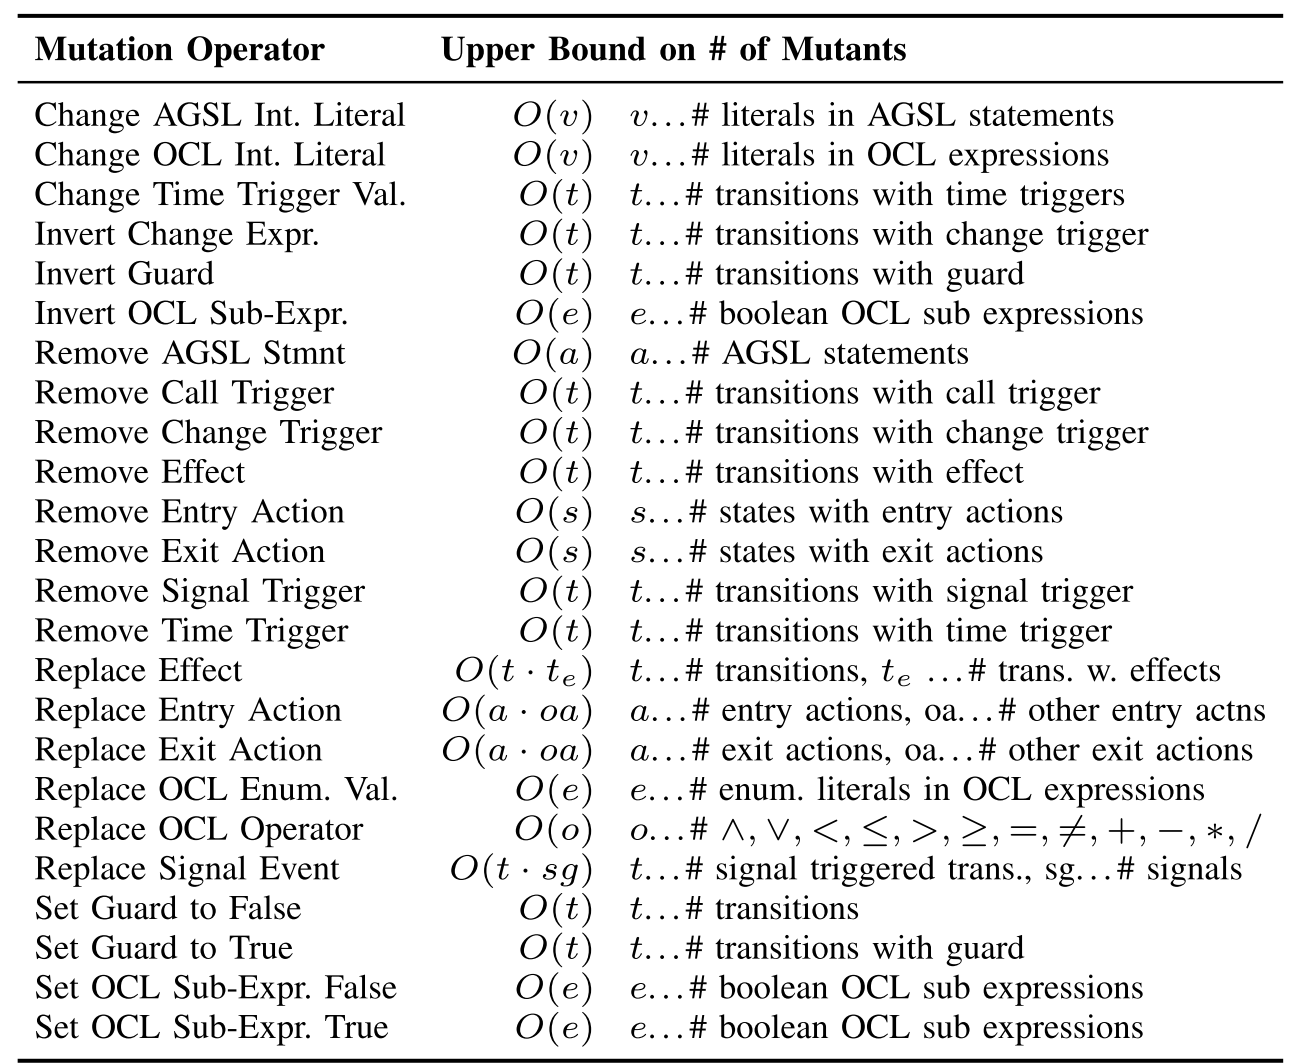
\includegraphics[width=0.6\textwidth]{images/aichernig2015}
%      \caption{Mutation operators introduced in \cite{Aichernig2015}.}
%\end{figure}
%
%%Test cases are generated by choosing a trace within the product graph starting from the initial state and ending at a fail state. Action systems usually describe non-deterministic behaviour, i.e. there can be multiple observable actions enabled at the same time and an implementation is allowed to choose among them. So, whenever there is a branch on observables in the product graph along the chosen trace to the fail state, this branch also is copied into the generated test case, yielding an adaptive test case.
%
%
%
%Model-based data mutation is not only applicable to UML models, in fact, Siavashi et al.~\cite{Siavashi2018} presented a model-based mutation testing approach for evaluating the authentication and authorization of web services in a multi-user context. The modeling of the web service and its security requirements are performed using an UPPAAL timed automata, the model is then mutated to create invalid behavior which is used for test generation to reveal faults in the SUT.
% 
%In model-based mutation testing (MBMT), the original test model is altered systematically by mutation operators creating multiple versions of a model, known as mutant models. The mutants can be used for automatic generation of invalid test inputs that are executed against the SUT. The goal in MBMT is to find whether any invalid tests can pass the testing, thus they can reveal unexpected behavior (i.e., a fault) in the SUT. Hence, MBMT can expose the mistakes that are caused by missing requirements or incorrect implementation.
%
%In the paper, authors model a web service, its users, and their authentication and authorization requirements. The model is then mutated to create invalid test inputs that target faults in the implementation of the web service. 
%
%Mutation testing extends the fault detection capabilities of MBT by exposing more vulnerabilities of systems. It changes a system's program or its specification, to create new versions of the system. 
%Mutation operators are rules that establish the mutants by altering the syntax of the program (or the specification). The generated tests exhibit altered inputs (including faulty inputs) and input sequences against the SUT. Hence the mutants allow testing of the SUT with invalid inputs. 
%
%The paper introduces eight mutation operators for timed automatas, five operators concern to action elements, and three to guard elements of the automata.
%
%\begin{table}[h!]
\begin{center}
\footnotesize
\begin{tabular}{|p{5cm}|p{10cm}|}
\hline
\textbf{Fault}&\textbf{Description}\\
\hline
Change Name of Actions (CN) & Replaces the name of an action with the name of other actions in the model. Thus, the expected sequence of the inputs to the implementation will be different..\\
Change Target of Actions (CT) & Changes the target location of an action to another location in the model. This operator breaks the flow of test inputs and violates the state of the model. Both input and output actions can be mutated by this operator.\\
Change Source of Actions (CS)& Changes the source location of an action to another location. Similar to CT, this operator mutates the sequence of input/outputs. \\
Remove Actions (RA)& randomly deletes one action at a time and creates a mutant. Omitting an action will manipulate the sequence of input/output actions.\\
Duplicate Actions (DA)& randomly copies an action in different parts of a model, thus alternates the sequence of inputs and outputs by repeating actions in unexpected states of the model.\\
Remove Guards (RG)& randomly selects an action and removes its guard. Actions that are mutated by RG will be always enabled.\\
Change Guards Logical Operators (CGL)& changes logical operators (i.e., ==, <=, >=, !=, < and >) in guards.\\
Change Guards Variables (CGV) & alters values of the variables that are used in guards and creates additional mutants that cannot be defined by other mutation operators\\
\hline
\end{tabular}
\end{center}
\caption{Fault Model from \cite{Siavashi2018}}
\label{table:faultModel:Siavashi}
\end{table}%

%
%%\textbf{MutRex: A Mutation-Based Generator of Fault Detecting Strings for Regular Expressions}
%
%Similarly, Arcaini et al.~\cite{Arcaini2017} proposed a model-fault-based approach for generating tests for regexes. The work is based on an automata representation of regexes that generates distinguishing strings exposing the faults introduced in mutated versions of a regex under test. The paper also introduces fault classes representing possible mistakes a user can make when writing a regex.
%
%The proposed tool, MutRex, first produces some mutants from a regex $r$ according to some fault classes representing common mistakes that are made when writing regexes; then, for each mutant $m$, it generates a string $s$ able to distinguish $m$ from $r$, i.e., a string that is evaluated differently in $r$ and $m$ (in terms of mutation testing, $s$ kills $m$). The set of generated strings is a test suite able to detect all the seeded faults.
%
%The authors identified three families of faults: \textit{single character faults}, \textit{character class faults} are respectively related to wrong uses of single characters and character classes, instead \textit{other faults} are related to wrong uses of the multiplicity and of the negation operator.
%
%\begin{table}[h]
%\caption{Mutation operators implemented by MutRex}
%\label{table:MutRex}
%\tiny
%\begin{tabular}{|p{3cm}|p{11cm}|}
%\hline
%\multicolumn{2}{|c|}{Single character faults}\\
%\hline
%Case Change CC & Regexes are case sensitive. However, a user could use them without being aware of this, or she could simply use the wrong case (either upper or lower). This operator mutates a regex r by changing the case of characters appearing in r: a mutant is created for each character of r not used in a character class, and a mutant is created for each character.\\
%Case Addition CA&This operator is similar to CC, but makes both lower and upper cases possible when only one of the two is used: for each character of the regex r not used in a character class it creates a mutant with the other case of the char added as alternative; for each character class, instead, the mutant adds as alternative a new character class having the extremes of the interval in the other case.\\
%Metachar to Char M2C& In a regex, some characters can be interpreted as metachars or chars depending on the context, and there is no mandatory special way to identify metachars. For example, character '-' is interpreted as a metachar only in character classes, otherwise it matches the normal dash character. A user may want to use a char c, but she could wrongly use c as metachar. This operator transforms a regex r containing a char c interpreted as a metachar in a regex r' in which c is interpreted as a char. Note that the way to mutate r depends on the metachar c: for example, M2C applied to '-' removes the character class where '-' is used.\\
%Char To Metachar C2M & In other cases, instead, the designer wants to use a metachar c, but, because of the context, c is interpreted as a simple char. This operator transforms a regex r containing a c interpreted as a char in a regex r' in which c is interpreted as a metachar. Similarly to M2C, the way to mutate r depends on the metachar c.\\
%\hline
%\multicolumn{2}{|c|}{Character class faults}\\
%\hline
%Character Class Creation CCC& Character classes are delimited by square brackets []. A user may want to use a character class and forgets (or ignores) the parentheses. Given a regex $r = c_{1}-c_{2}$, the operator mutates $r$ in $r'= [c_{1} - c_{2}] $.\\
%Character Class Addition CCA&The user could have forgotten a given interval in a set of character classes. Given a regex $r = [cc_1 ... cc_n]$, the operator creates a mutant $r' = [cc_1 ... cc_n cc_{new} ]$ for each $cc_new$ not present in r; $cc_{new}$ can be a-z, A-Z,or 0-9.\\
%Range Modification RM&The user could have specified the operator produces a mutant in which $c_1$ or $c_2$ is increased a too tight or too broad interval. Given a regex $r = [c_1 - c_2]$, or decreased (if it is still a valid char). \\
%Character Class Restriction CCR& The user could have written a regex that is too permissive since it accepts characters that should not. Given a regex $r =[cc_1 ... cc_n]$, the operator creates a mutant $r' = [cc_1 ... cc_{i-1}cc{i+1} ... cc_n]$ for each $cc_i$ (i.e., it removes an interval from the character class).\\
%Prefix Addition PA& Sometimes all the characters of a string $s$ satisfy some constraints, except for the first character in $s$ that must satisfy additional constraints; for example, identifiers in most programming languages cannot start with a number. This mutation operator, given a repeat expression regex $r =[cc_1, ..., cc_n]m$ (being $m$ the multiplicity), introduces a prefix that is one of the different character classes $cc_1, ..., cc_n$ used in $r$. The obtained mutants are as follows: $[cc_1][cc_1, ..., cc_n]m, [cc_2][cc_1, ..., cc_n]m, ..., [cc_n][cc_1, ..., cc_n]m$.\\
%Character Class Negation CCN& Regex [ˆ$cc_1 ... cc_n]$ matches any character that is not listed in the character classes $cc_1, ..., cc_n$. The designer could have forgotten the ˆ symbol and written $[cc_1 ... cc_n]$. CCN introduces symbol ˆ it creates a mutant in which all the character classes are excluded (i.e, [ˆ$cc_1 ... cc_n$]), and a mutant for each character class $cc_i$ in which only $cc_i$ is excluded (i.e, $[cc1] | ...| [$ˆ$cc_i] | ...| [cc_n])$.\\
%
%Negated Character Class to Optional NCCO& Another common error regarding the use of a negated character class [ˆcc] is that it requires 'to match a character that is not listed' and not 'to not match what is listed'. Therefore, a negated character class still requires to match a character. A user could misunderstand the semantics of the operator, thinking that it simply excludes the character; in some cases, for example at the end a word, she could be interested in accepting also no character. Operator NCCO makes ˆ optional, i.e., it mutates [ˆcc]in[ˆcc]?\\
%\hline
%\multicolumn{2}{|c|}{
%Other faults}\\
%\hline
%Negation Addition NA&In a regex $r = r_1r_2 ...r_n$, the user could forget a negation ˆ. The operator creates a mutant adding a negation wherever possible in $r$, i.e., ˆ$r_1r_2 ...rn, r_1$ˆ$r_2r_n, ..., r1r2 ... $ˆ$r_n$. \\
%Quantifier Change QC&The user could have used the wrong cardinality. The operator mutates each simple repeat quantifier in another simple quantifier; moreover, for each user-defined quantifier, it creates a mutant in which $n$ (or $m$) is increased and a mutant in which it is decreased.
%Example\\
%\hline
%\end{tabular}
%\end{table}
%
%
%A mutant $m$ of a regex $r$ can modify the accepted language in four ways: 
%\begin{itemize}
%  \item Arbitrary edit: some words are added to the language and other words are removed.
%  \item Generalization: some words are added to the language and no word is removed.
%  \item Specialization: some words are removed from the language and no word is added.
%  \item Equivalent: the mutant is equivalent and so the two languages are the same.
%\end{itemize}
%
%
%%\textbf{Combinatorial mutation approach to web service vulnerability testing based on SOAP message mutations}
%
%In a different context, Li et al.~\cite{Li2012} proposed a model-based combinatorial mutation approach based on SOAP messages for Web service vulnerability testing.
%The technique presented in the paper consists of (1) analyzing the web service methods and identify all the associated web service methods. (2) Invoke different sets of mutation operators according to the perturbation policy on the SOAP messages (XML documents) by parsing the WSDL files, and then (3) call the appropriate combinatorial testing approach to generate combinatorial test cases.
%
%The XML model-based approach presents the following two perturbation policies: data value and interaction perturbations. Both perturbation policies directly act on the SOAP messages. The former one modifies values in SOAP messages according to their data types while the latter one may consider the data values and data relationships. Part of the mutation operators bear double effects of data value and interaction perturbations.
%
%The following mutation operators were introduced:
%
%\begin{figure}[h]
%  \centering
%    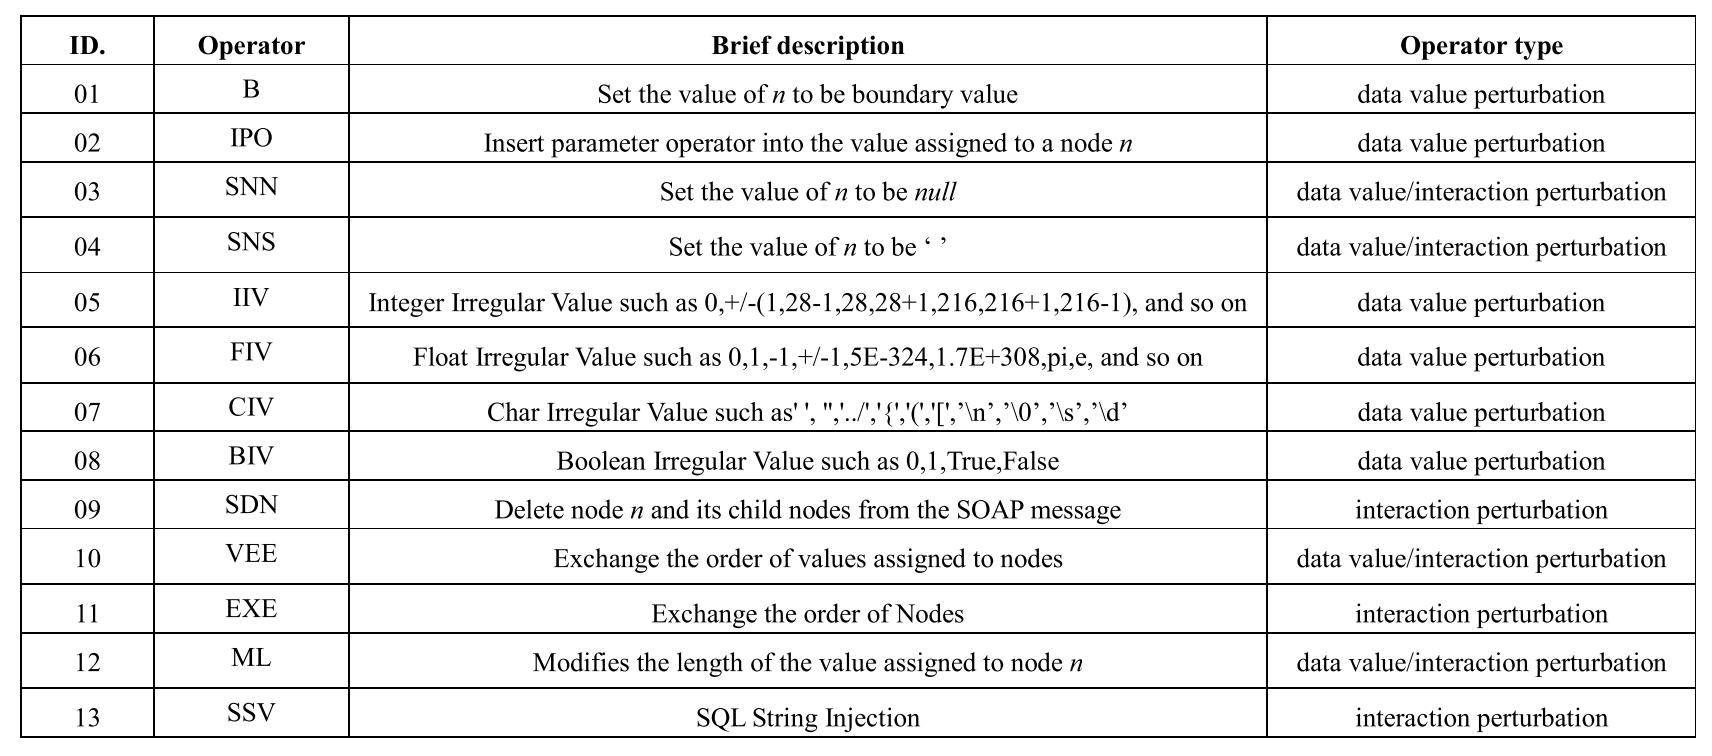
\includegraphics[width=\textwidth]{images/li2012}
%      \caption{Combinatorial mutation approach to web service vulnerability testing based on SOAP message mutations \cite{Li2012}}
%\end{figure}
%
%%\textbf{Worst-input mutation approach to web services vulnerability testing based on SOAP messages}
%
%Similarly, Chen et al.~\cite{Chen2014} introduced a model-based mutation approach for testing web service vulnerability of SOAP messages. 
%
%The method involves partitioning the input domain into sub-domains according to the number and type of SOAP message parameters in the TCFN (test case farthest neighbor) and then selecting the candidate test case whose distance is the farthest from all executed test cases and applying it to test the Web service.
%
%Web service vulnerability refers to flaws in the service that threaten the security of the computer system, for example, memory leaks, buffer overflows, and cross-boundary access (where memory variables access areas outside their defined scope)
%
%SOAP is a message protocol based on an XML document, which forms the basis of the mutation object. The paper introduces 15 mutation operators for SOAP parameters types combined with Web service features.
%
%\begin{figure}[h]
%  \centering
%    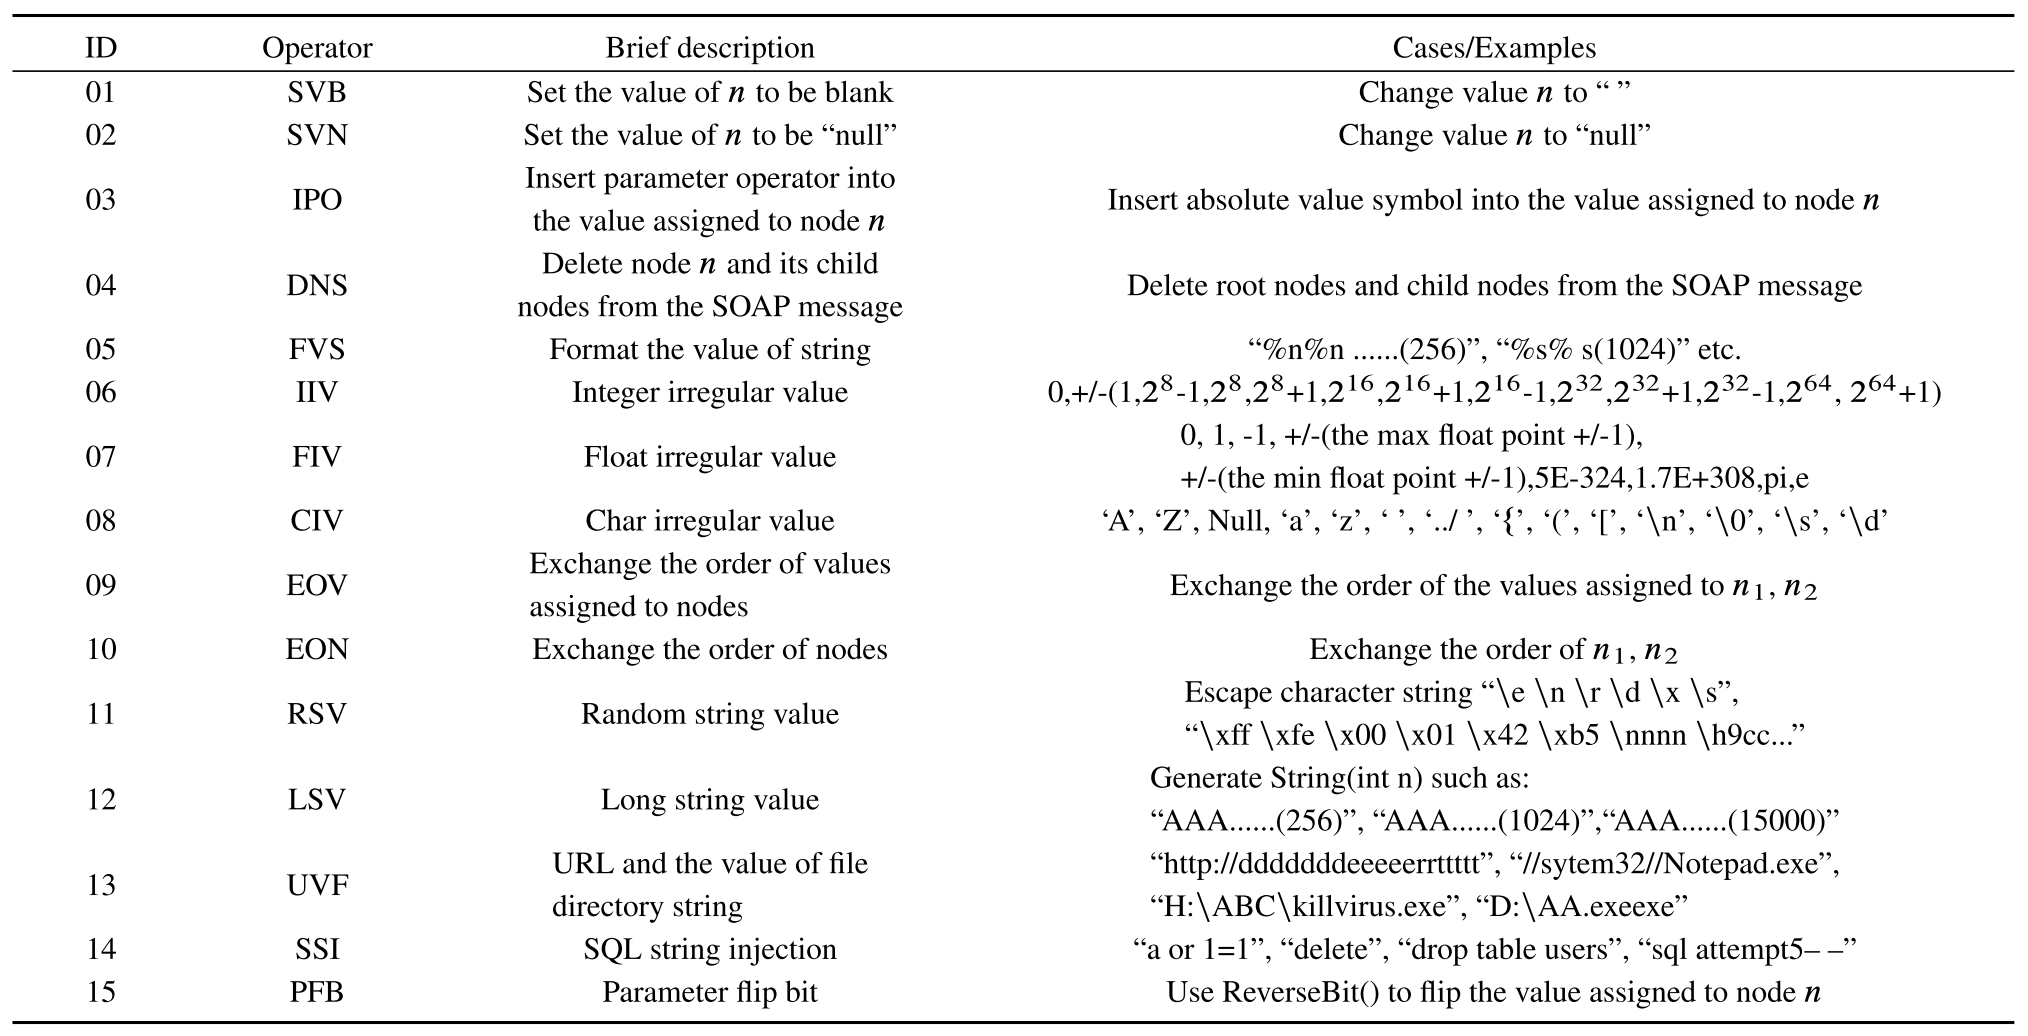
\includegraphics[width=0.8\textwidth]{images/chen2014}
%      \caption{SOAP messages mutation operators.}
%\end{figure}
%
%
%\subsubsection{Search-based data mutation}
%
%Search-based data mutation relies on an evolutionary algorithm to perform model-based data mutation and optimize multiple objectives:  
%cover all the classes of the data-model, cover all the possible faults of the fault model, cover all the clauses of the input/output constraints,
%maximise code coverage~\cite{di2015evolutionary}.
%The coverage of each objective is encoded by means of boolean arrays; this information is used to select a minimal set of inputs that maximize the coverage of the different objectives.
%At every iteration, the evolutionary algorithm keeps only inputs that contribute to increase the coverage of at least one of the objectives (e.g., inputs that cover one instruction not covered by other inputs).
%
%An additional source of information concerning the adoption of fuzzing and grammar-based approaches to perform test input generation is the \emph{Fuzzing Book}~\cite{fuzzingbook2019:GrammarFuzzer}.
%
%
%\subsection{Automated Detection of Equivalent and Redundant Mutants}
%\label{sec:dataequivalent}
%
%Data-driven mutation operators may lead to the generation of both equivalent and redundant mutants.
%In the data-driven context, equivalent mutants consist of modified data (i.e., data altered by means of mutation operators) that do not lead to any noticeable difference in the output of the SUT with respect to the original version of the data.
%Please note that an equivalent mutant differs in content from the original data (i.e., the data chunk has been altered).
%The possible reasons why a mutant may not lead to noticeable differences in the output of the SUT are three. First, changes may go unnoticed because they alter portions of the data that is not read by the SUT. This includes cases in which mutations alter the structure of the input data in such a way that the resulting mutated data is different from the original but still respect the data format. This might happen, for example, when a mutation operator swaps the CDATA section of an XML file and the SUT ignores CDATA content. Second, mutations may alter some of the outputs of the SUT but the test suite oracles ignore that portion of the output. This might happen in a data acquisition system that copies the data payload of network packets in a database; in such a context, a data mutation that alters the message and update the packet checksum might go unnoticed because the SUT would simply copy the message content to the database and the test suite may simply check if the database contains a new message. Third, mutations may alter valid existing data but produce data that is still valid. This often reflect a poor choice of mutation operators; indeed, the selected mutation operators should guarantee to introduce a fault in the data exchanged by the system.
%
%
%Redundant mutants cause the same failures in the test suite. Two are the reasons for redundant mutants. First, the mutations alter different instances of a same data structure in the same way (e.g., delete a message in a sequence). Second, the mutations alter data chunks that are ignored by the oracles of the test suite.
%
%Concrete examples of equivalent and redundant mutants are provided in Figure~\ref{fig:data:quivalent}. In Figure~\ref{fig:data:quivalent}, \emph{Mutation 2} leads to an equivalent mutant since it generates a timestamp that is just one millisecond in the past, which is legal for the system under test. The value 2 for a timestamp, instead, leads to a failure because is considered too much in the past (see \emph{Mutation 1}). To address this problem, engineers should have configured the timestamp field to be mutated by a boundary condition operator (which generates values out of valid range) instead of a bit flipping operator. \emph{Mutation 3}  and \emph{Mutation 4}, instead, are redundant because they both generate a timestamp in the future (under the assumption that \emph{1584889773} captures the current time).
%
%\begin{figure}[h]
%  \centering
%    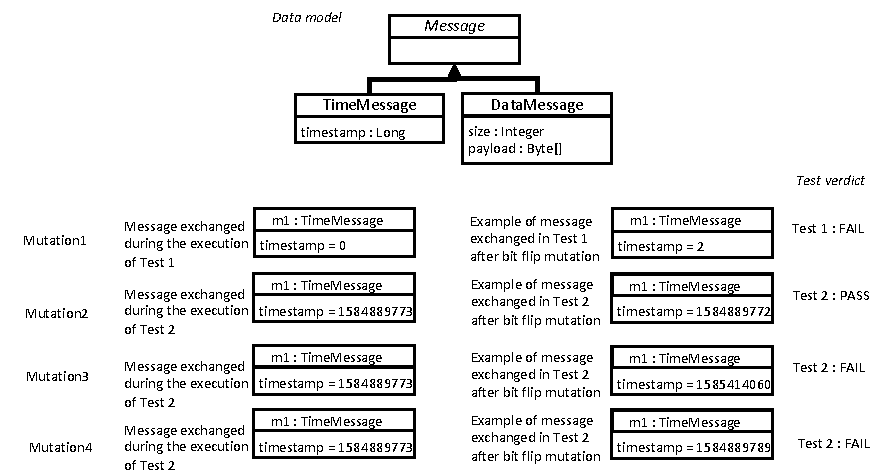
\includegraphics{images/DataDrivenEquivalent}
%      \caption{Examples of data-driven mutations leading to equivalent and redundant mutants.}
%      \label{fig:data:quivalent}
%\end{figure}
%
%Literature lacks approaches to directly target equivalent and redundant mutants. However, some of the solutions implemented in existing data mutation approaches might limit the presence of equivalent and redundant mutants. We observe three main solutions: (1) driving mutations by means of code-coverage, (2) driving mutations by means of coverage of model structure, and (3) use of model-based oracles.
%
%Code-coverage-driven mutations are the ones implemented by many automated fuzzers such as 
%MoWF~\cite{pham2016model} and AFL~\cite{gutmann2016fuzzing}.
%MoWF aims to generate mutated data that triggers the execution of specific code locations. This is done by combining symbolic execution and meta-heuristic search.
%Since each mutated input triggers a different code location, MoWF, in principle, should always lead to mutated inputs that make the software behave differently than with the original input or with other data mutants. However, it does not ensure that the changes in the internal behaviour of the software are reflected in one of its observable outputs.
%Similarly to MoWF, AFL generates inputs that trigger different code locations. The main difference is that it does not target only specific code locations but it aims to exercise all the branches of the program. 
%Similarly to MoWF, AFL does not guarantee that changes in the internal behaviour of the software are reflected in one of its observable outputs.
%Similarly to AFL, any approach relying on meta-heuristic search that include coverage objectives in the fitness function (e.g.,~\cite{di2015evolutionary}) can limit the presence of equivalent and redundant mutants.
%
%
%The coverage of the model structure enables the generation of mutations targeting different portions of a given data model.
%For example, \emph{pFuzzer} generates valid inputs that cover diverse sets of lexical and syntactical features.
%Other approaches~\cite{di2015generating} generate mutants that target different elements of the data structure.
%By targeting different elements of the data, the generated mutants are unlikely to be redundant or equivalent. However, they do not ensure that such differences are reflected in the SUT observable outputs.
%
%
%Model-based oracles, such as OCL constraints capturing expected outputs (e.g., error messages expected in the presence of a specific change of the data) enable the generation of mutants that are not equivalent and not redundant. For example, by ensuring that each mutant affects a model element referenced in a different OCL constraint and that the constraint is evaluated to true, model-based mutation approaches can guarantee that the data mutations lead to observable changes in the SUT output~\cite{di2015generating}.
%
%
%\newcommand{\ONMO}{\mathit{overall}\ \# \mathit{of}\ \mathit{mutation} \ \mathit{operators}}
%\newcommand{\NMOA}{\# \mathit{of}\ \mathit{mutation} \ \mathit{operators} \ \mathit{applied}}
%
%
%\subsection{Analysis of Mutation Testing Results and Mutation Score Calculation}
%\label{sec:data:mutationscore}
%
%In the data-driven mutation testing process, the outcome of the activity \emph{Analyze Results} (see Figure~\ref{fig:data:process}) is a mutation score that is based on
%the percentage of mutants being killed and the percentage of mutation operators applied. 
%The former enables data-driven mutation to achieve objective O1 in Section~\ref{sec:dataProcess}, the latter objective O2. 
%The mutation score can be computed as a weighted average of the percentage of mutants being killed and the percentage of mutation operators applied, according to the following formula
%
%\begin{equation}
%Score=w_{O1} \frac{\# \ \mathit{of}\ \mathit{killed} \ \mathit{mutants}}{\mathit{overall} \# \mathit{of}\ \mathit{mutants}} + w_{O2} \frac{\# \mathit{of}\ \mathit{mutation} \ \mathit{operators} \ \mathit{applied}}{\mathit{overall} \# \mathit{of}\ \mathit{mutation} \ \mathit{operators}}
%\label{f:mutation:score}
%\end{equation}
%
%Where $w_{O1}$ and $w_{O2}$ capture the importance of the objectives O1 and O2, respectively. We assume $w_{O1}$ + $w_{O2} = 1$. In case objective $w_{O1}$ and $w_{O2}$ have the same importance, they should be set to $0.5$. In the case of safety-critical systems, the mutation score should be equal to 1.
%
%In formula \ref{f:mutation:score}, the $\mathit{overall}\ \# \mathit{of}\ \mathit{mutants}$ corresponds to the number of test executions in which at least one data object have been altered through mutation. We refer to such test executions as \emph{mutated test executions}.
%The $\# \ \mathit{of}\ \mathit{killed} \ \mathit{mutants}$ corresponds to the number of \emph{mutated test executions} that either failed or during which a redundancy mechanisms has been activated to handle the mutated data.
%
%The $\ONMO$ corresponds with the number of different mutations that can be applied to the data, according to the data model. It depends on the strategy adopted to select the items to be mutated.
%% and may vary based on the strategy adopted to perform data mutation.
%For approaches relying on \textbf{UML models}, one possibility is to follow the approach of Di Nardo et al.~\cite{di2015generating}, which consists of mutating every model element (e.g., class or class attribute in the class diagram capturing the data model) with every mutation operator that is applicable to the specific model element, according to the fault model captured in the class diagram (see Section~\ref{sec:data_operators}).
%The $\ONMO$ (ONMO) could be thus computed as the sum of the number of applicable mutation operators for ever every model element.
%The $\NMOA$, (NMOA) consequently, should capture the number of mutations that were performed. In the approach of Di Nardo et al.~\cite{di2015generating}, NMOA corresponds to the number of model elements for which at least one instance had been mutated. 
%
%For the computation of ONMO and NMOA, a strategy similar to the one presented by Di Nardo et al. can be used also in the case of approaches relying on \textbf{grammars} or \textbf{block models}. Indeed, also for these two types of approaches, data mutation is performed by means of a set of mutation operators that are applied in the presence of specific data types. 
%These data types correspond to the production rules of the grammar or the blocks defined in the block model. 
%Approaches that do \textbf{not require an input model} typically work at the bit/byte level. In these cases, ONMO might be calculated as the number of available operators, or
%as the number of bit/bytes in the inputs multiplied by the number of applicable mutation operators.
%
%
%Moreover, data njection has been usually used to asses the robustenss of software here we apply to assess the test suite with respct to interoperability faults.
%%this is the first work relying on data fault injection procedures to perform mutation analysis.
